%-----------------------------------------------------------------------------%
\chapter{\babEmpat}
%-----------------------------------------------------------------------------%

%-----------------------------------------------------------------------------%
\section{Hasil Pengujian Tuning Hypervisor KVM dengan Kompresi Video}
%-----------------------------------------------------------------------------%

%-----------------------------------------------------------------------------%
\subsection{Konfigurasi Default}
%-----------------------------------------------------------------------------%
\begin{figure}
    \centering
    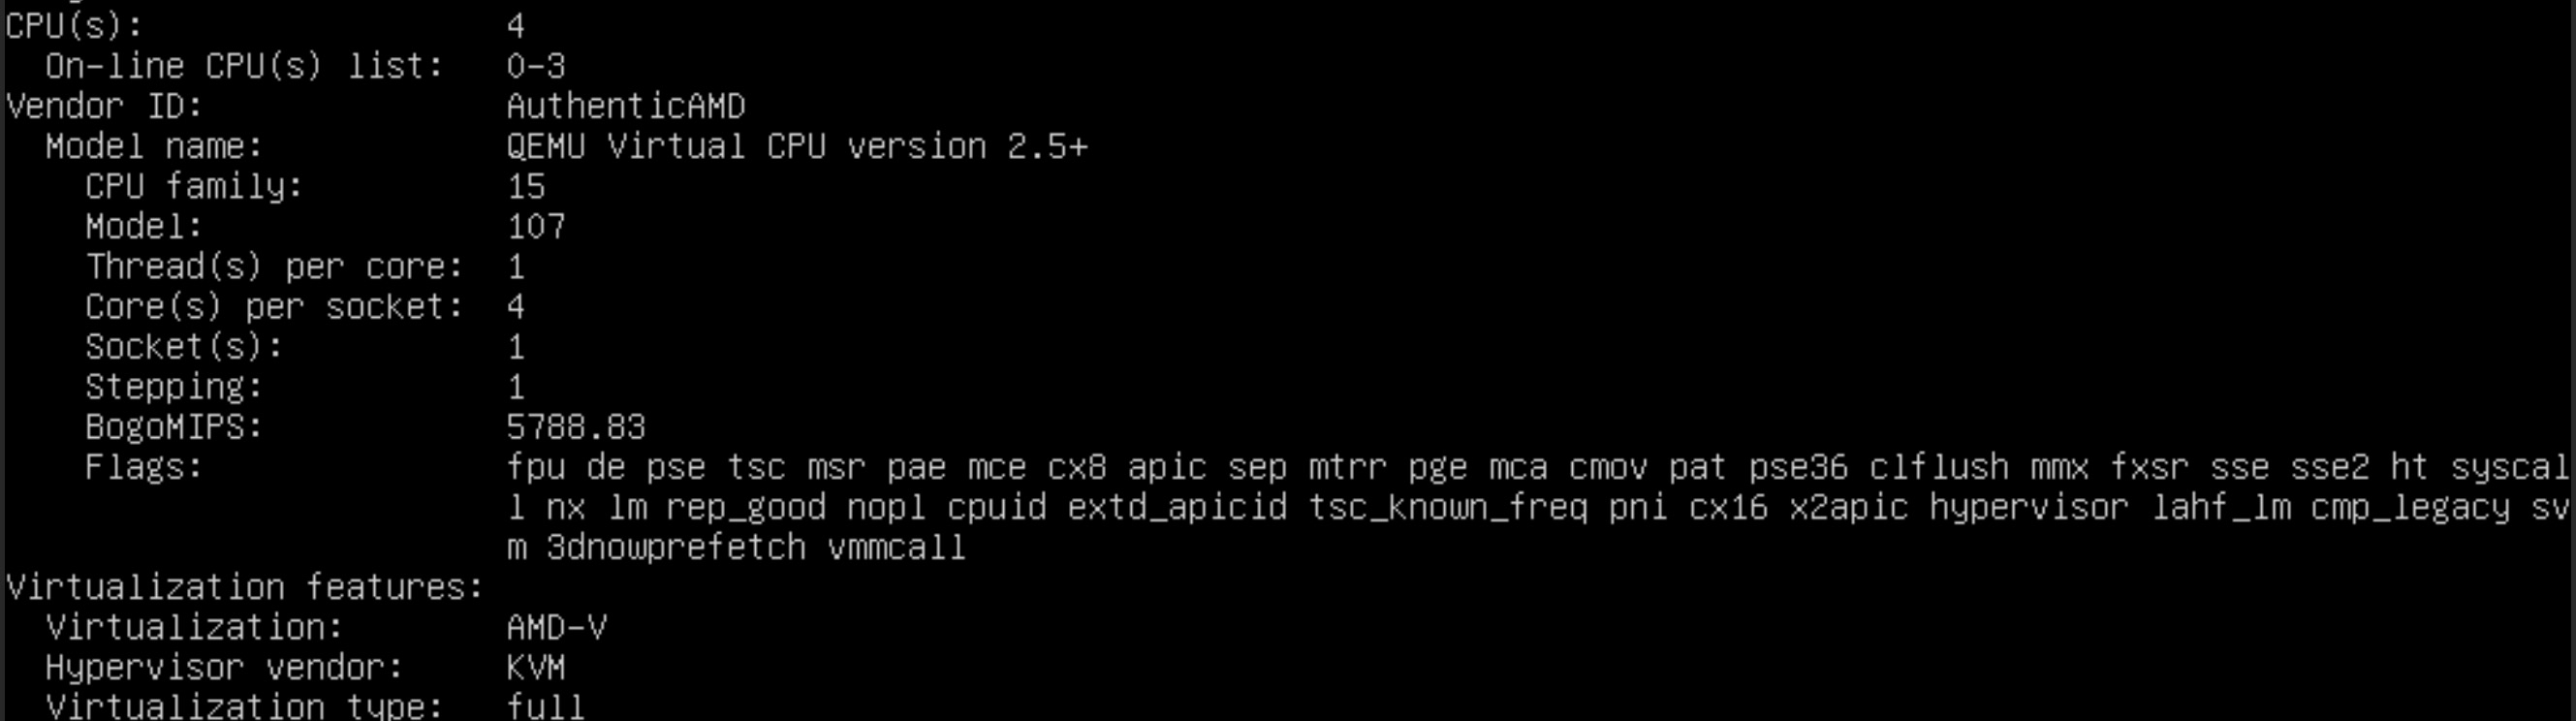
\includegraphics[width=1\textwidth]
    {assets/pics/video-compression-test/lscpu_original.jpeg}
    \caption{\texttt{lscpu} Konfigurasi Default}
    \label{fig:lscpu_video_compression_test_original}
\end{figure}

\begin{figure}
    \centering
    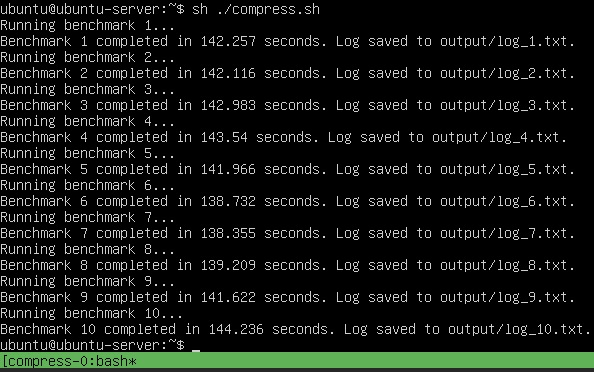
\includegraphics[width=1\textwidth]
    {assets/pics/video-compression-test/original.jpeg}
    \caption{Test Kompresi Video dengan Konfigurasi Default}
    \label{fig:video_compression_test_original}
\end{figure}

\begin{figure}
    \centering
    \begin{tikzpicture}
        \begin{axis}[
            xbar,
            bar width=12pt,
            xlabel={Detik},
            ytick=data,
            nodes near coords,
            nodes near coords align={horizontal},
            symbolic y coords={run 1,run 2,run 3,run 4,run 5,run 6,run 7,run 8,run 9,run 10},
            enlarge y limits=0.2,
            enlarge x limits=0.05,
            width=\textwidth,
            height=0.4\textheight,
            xmin=0,
            xmax=160
        ]
        \addplot [fill=black] coordinates {
            (142.257,run 1) 
            (142.116,run 2) 
            (142.983,run 3) 
            (143.54,run 4) 
            (141.966,run 5)
            (138.732,run 6) 
            (138.355,run 7)
            (139.209,run 8) 
            (141.622,run 9) 
            (144.236,run 10)
        };
        \end{axis}
    \end{tikzpicture}
    \caption{Grafik Tes Kompresi Video dengan Konfigurasi Default}
    \label{fig:video_compression_test_original_graph}
\end{figure}


%-----------------------------------------------------------------------------%
\subsection{Konfigurasi dengan SSSE3}
%-----------------------------------------------------------------------------%
\begin{figure}
    \centering
    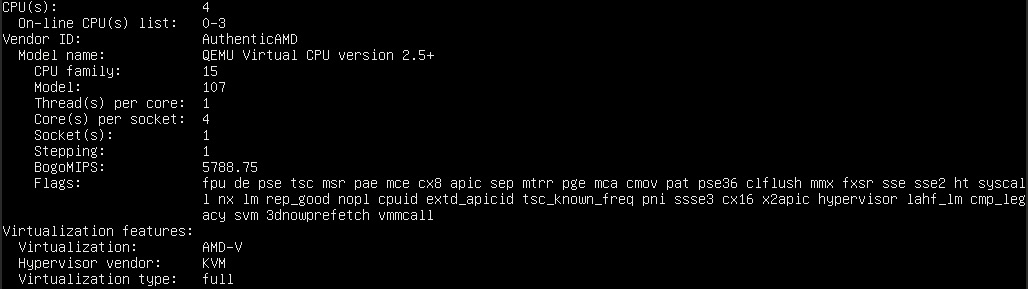
\includegraphics[width=1\textwidth]
    {assets/pics/video-compression-test/lscpu_ssse3.jpeg}
    \caption{\texttt{lscpu} Konfigurasi SSSE3}
    \label{fig:lscpu_video_compression_test_ssse3}
\end{figure}

\begin{figure}
    \centering
    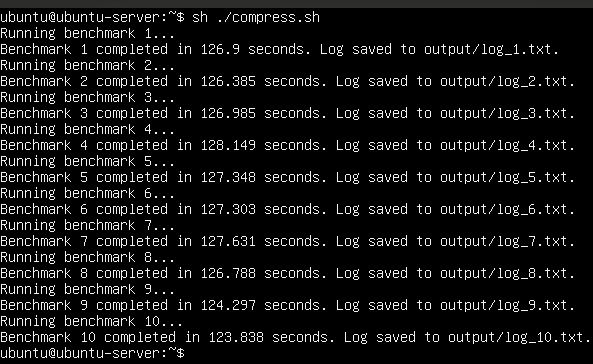
\includegraphics[width=1\textwidth]
    {assets/pics/video-compression-test/ssse3.jpeg}
    \caption{Test Kompresi Video dengan Konfigurasi SSSE3}
    \label{fig:video_compression_test_ssse3}
\end{figure}

%-----------------------------------------------------------------------------%
\subsection{Konfigurasi dengan SSE4.1}
%-----------------------------------------------------------------------------%
\begin{figure}
    \centering
    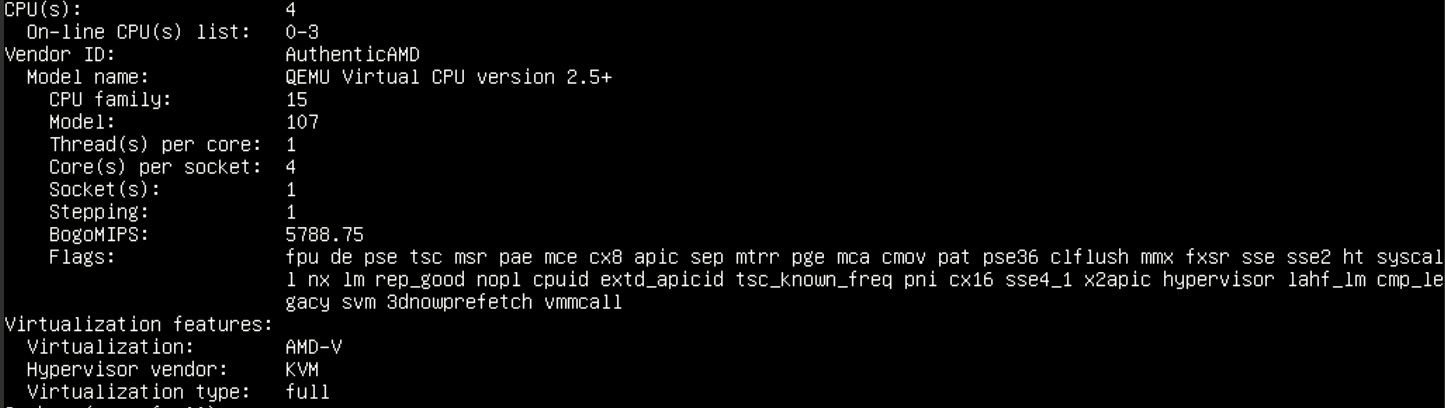
\includegraphics[width=1\textwidth]
    {assets/pics/video-compression-test/lscpu_sse4.1.jpeg}
    \caption{\texttt{lscpu} Konfigurasi SSE4.1}
    \label{fig:lscpu_video_compression_test_sse4.1}
\end{figure}

\begin{figure}
    \centering
    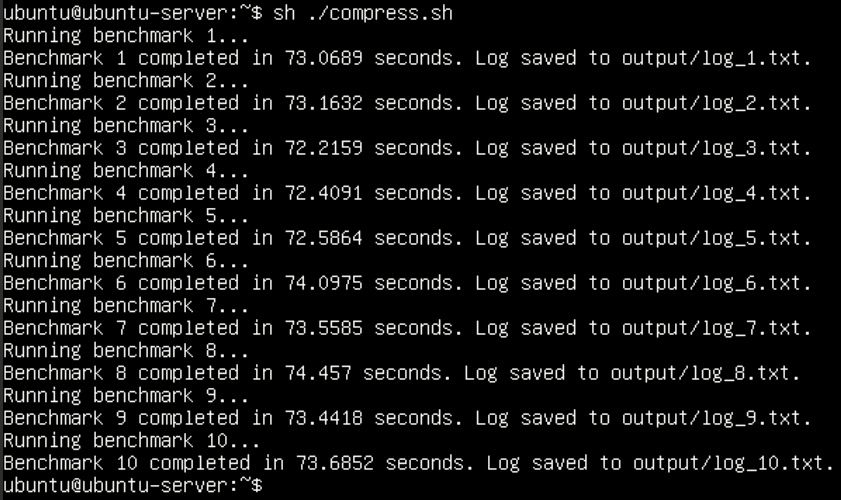
\includegraphics[width=1\textwidth]
    {assets/pics/video-compression-test/sse4.1.jpeg}
    \caption{Test Kompresi Video dengan Konfigurasi SSE4.1}
    \label{fig:video_compression_test_sse4.1}
\end{figure}

%-----------------------------------------------------------------------------%
\subsection{Konfigurasi dengan SSE4.2}
%-----------------------------------------------------------------------------%
\begin{figure}
    \centering
    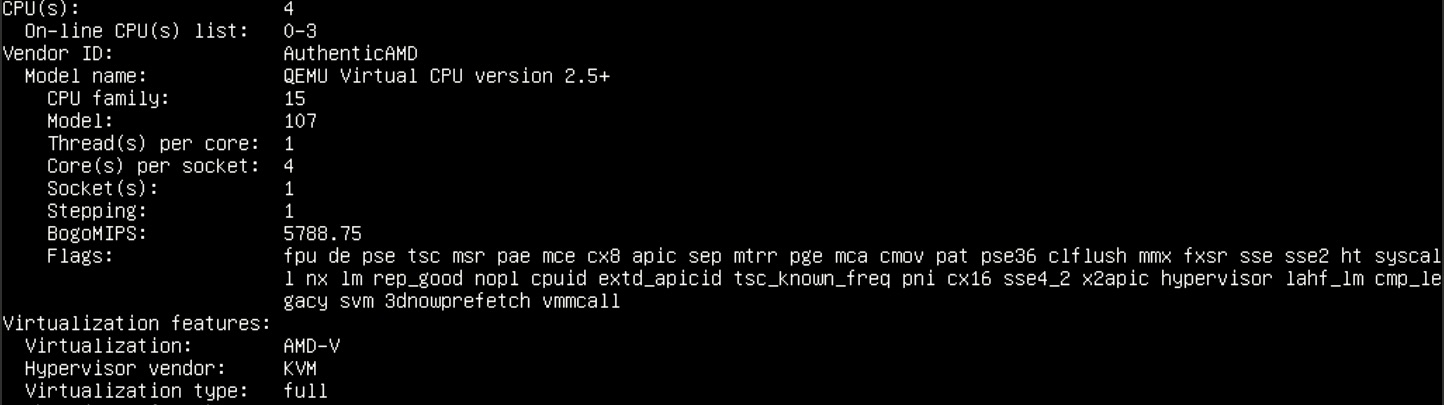
\includegraphics[width=1\textwidth]
    {assets/pics/video-compression-test/lscpu_sse4.2.jpeg}
    \caption{\texttt{lscpu} Konfigurasi SSE4.2}
    \label{fig:lscpu_video_compression_test_sse4.2}
\end{figure}

\begin{figure}
    \centering
    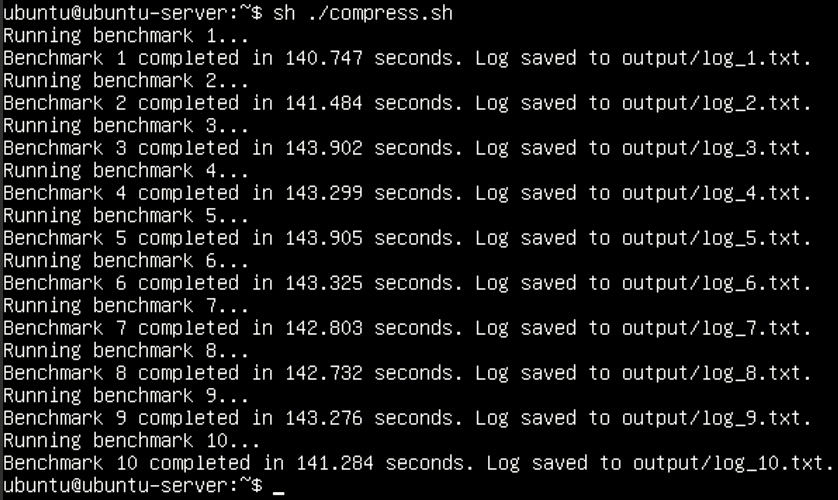
\includegraphics[width=1\textwidth]
    {assets/pics/video-compression-test/sse4.2.jpeg}
    \caption{Test Kompresi Video dengan Konfigurasi SSE4.2}
    \label{fig:video_compression_test_sse4.2}
\end{figure}

%-----------------------------------------------------------------------------%
\subsection{Konfigurasi dengan SSE4a}
%-----------------------------------------------------------------------------%
\begin{figure}
    \centering
    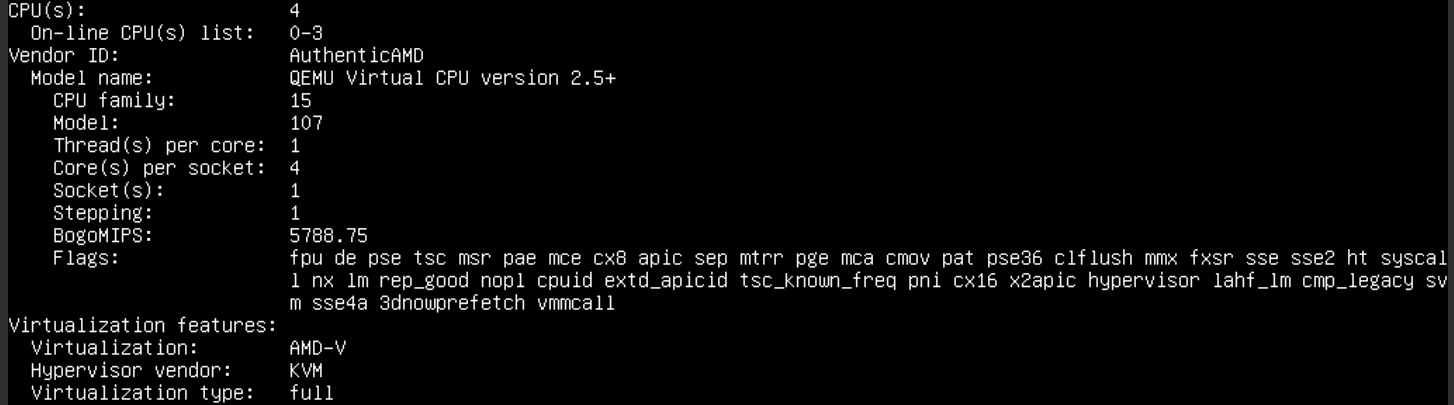
\includegraphics[width=1\textwidth]
    {assets/pics/video-compression-test/lscpu_sse4a.jpeg}
    \caption{\texttt{lscpu} Konfigurasi SSE4a}
    \label{fig:lscpu_video_compression_test_sse4a}
\end{figure}

\begin{figure}
    \centering
    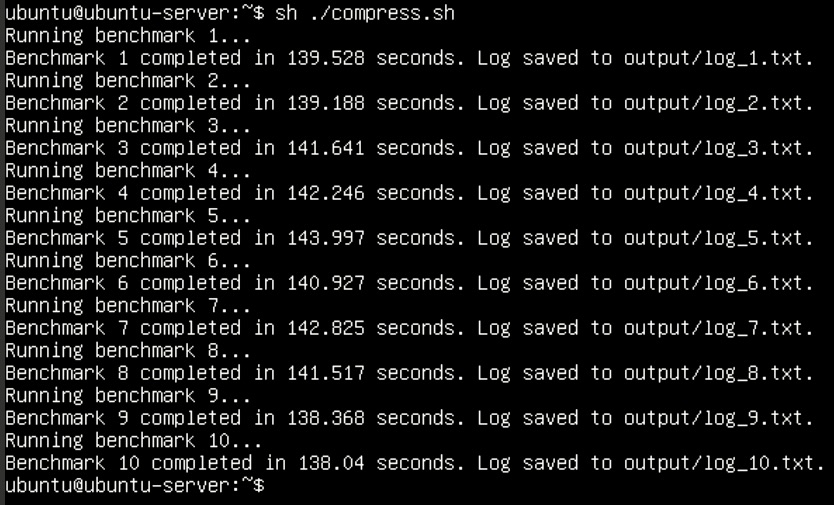
\includegraphics[width=1\textwidth]
    {assets/pics/video-compression-test/sse4a.jpeg}
    \caption{Test Kompresi Video dengan Konfigurasi SSE4a}
    \label{fig:video_compression_test_sse4a}
\end{figure}

%-----------------------------------------------------------------------------%
\subsection{Konfigurasi dengan SSSE3 + SSE4.1}
%-----------------------------------------------------------------------------%
% \begin{figure}
%     \centering
%     \includegraphics[width=1\textwidth]
%     {assets/pics/video-compression-test/lscpu_ssse3,sse4.1.jpeg}
%     \caption{\texttt{lscpu} Konfigurasi SSSE3 + SSE4.1}
%     \label{fig:lscpu_video_compression_test_ssse3,sse4.1}
% \end{figure}

\begin{figure}
    \centering
    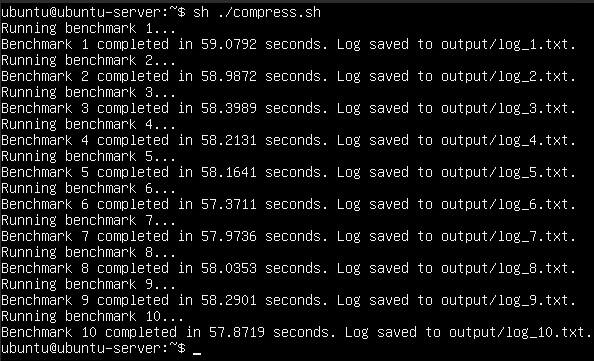
\includegraphics[width=1\textwidth]
    {assets/pics/video-compression-test/ssse3,sse4.1.jpeg}
    \caption{Test Kompresi Video dengan Konfigurasi SSSE3 + SSE4.1}
    \label{fig:video_compression_test_ssse3,sse4.1}
\end{figure}

%-----------------------------------------------------------------------------%
\subsection{Konfigurasi dengan SSSE3 + SSE4.2}
%-----------------------------------------------------------------------------%
\begin{figure}
    \centering
    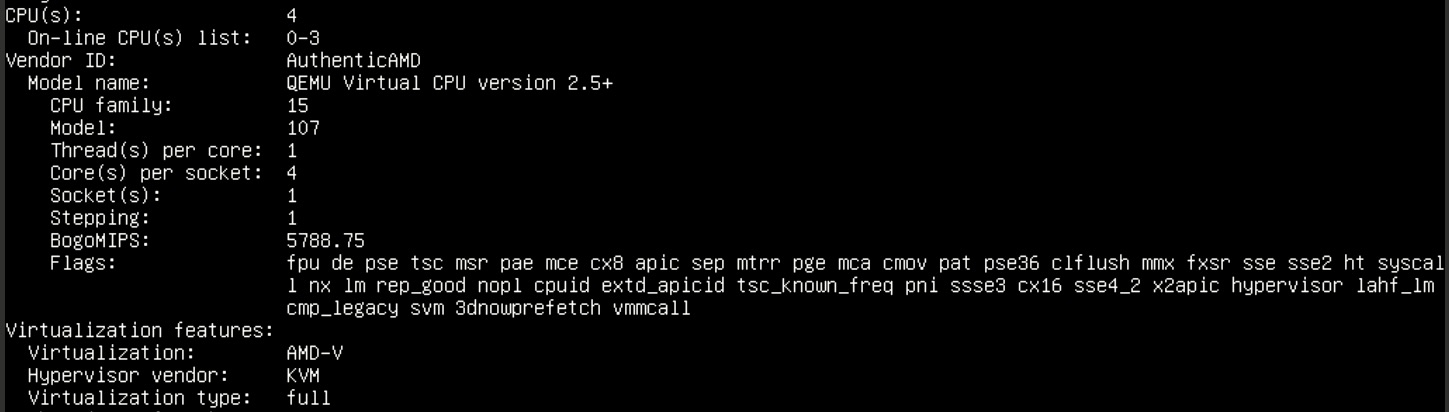
\includegraphics[width=1\textwidth]
    {assets/pics/video-compression-test/lscpu_ssse3,sse4.2.jpeg}
    \caption{\texttt{lscpu} Konfigurasi SSSE3 + SSE4.2}
    \label{fig:lscpu_video_compression_test_ssse3,sse4.2}
\end{figure}

\begin{figure}
    \centering
    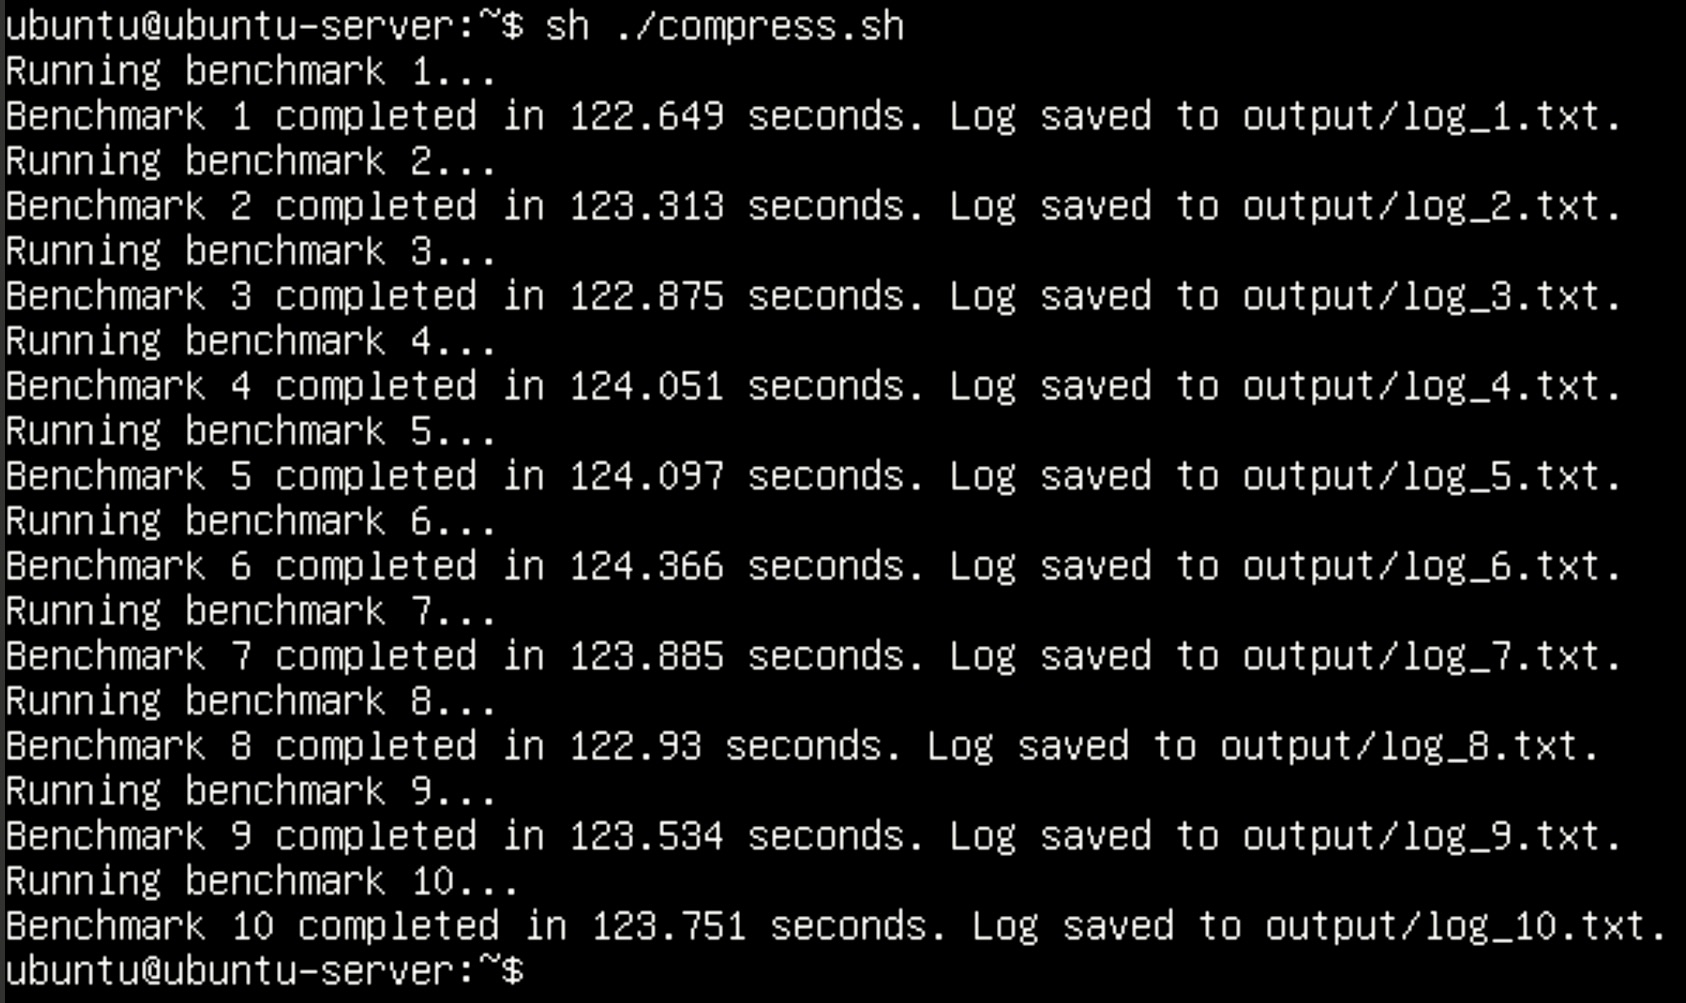
\includegraphics[width=1\textwidth]
    {assets/pics/video-compression-test/ssse3,sse4.2.jpeg}
    \caption{Test Kompresi Video dengan Konfigurasi SSSE3 + SSE4.2}
    \label{fig:video_compression_test_ssse3,sse4.2}
\end{figure}

%-----------------------------------------------------------------------------%
\subsection{Konfigurasi dengan SSSE3 + SSE4a}
%-----------------------------------------------------------------------------%
\begin{figure}
    \centering
    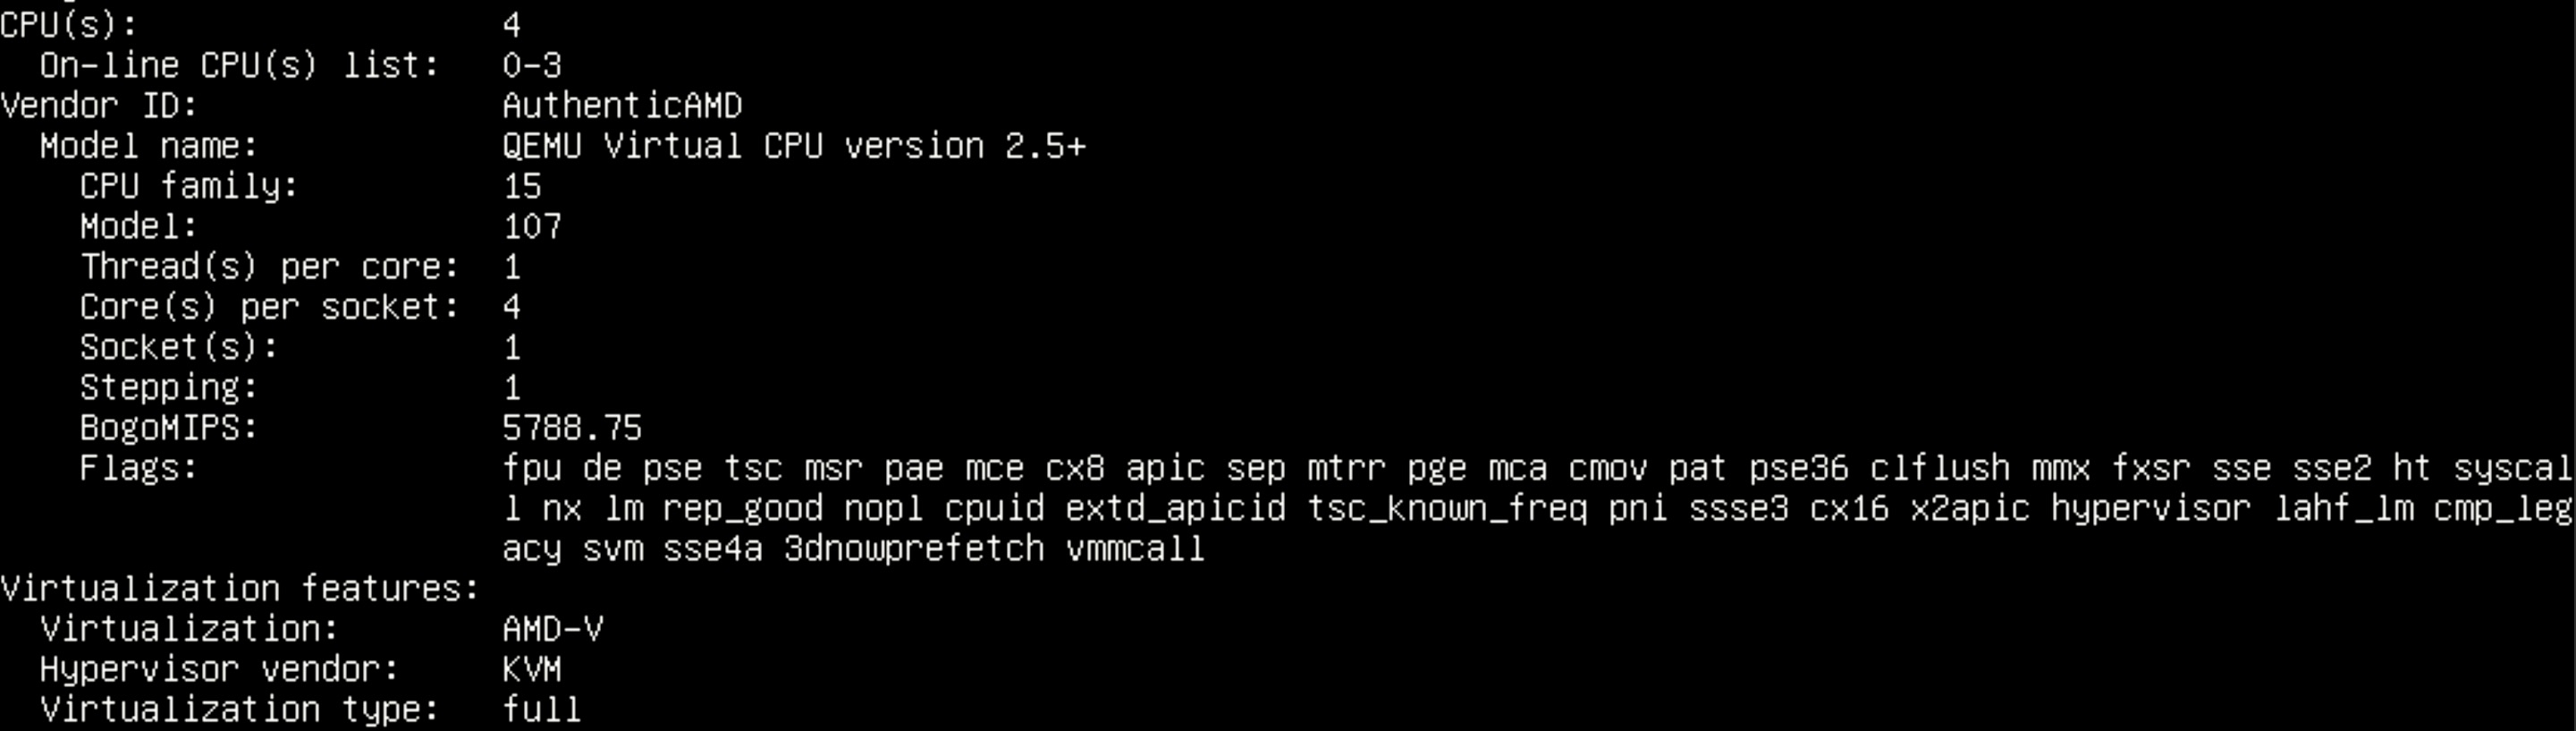
\includegraphics[width=1\textwidth]
    {assets/pics/video-compression-test/lscpu_ssse3,sse4a.jpeg}
    \caption{\texttt{lscpu} Konfigurasi SSSE3 + SSE4a}
    \label{fig:lscpu_video_compression_test_ssse3,sse4a}
\end{figure}

\begin{figure}
    \centering
    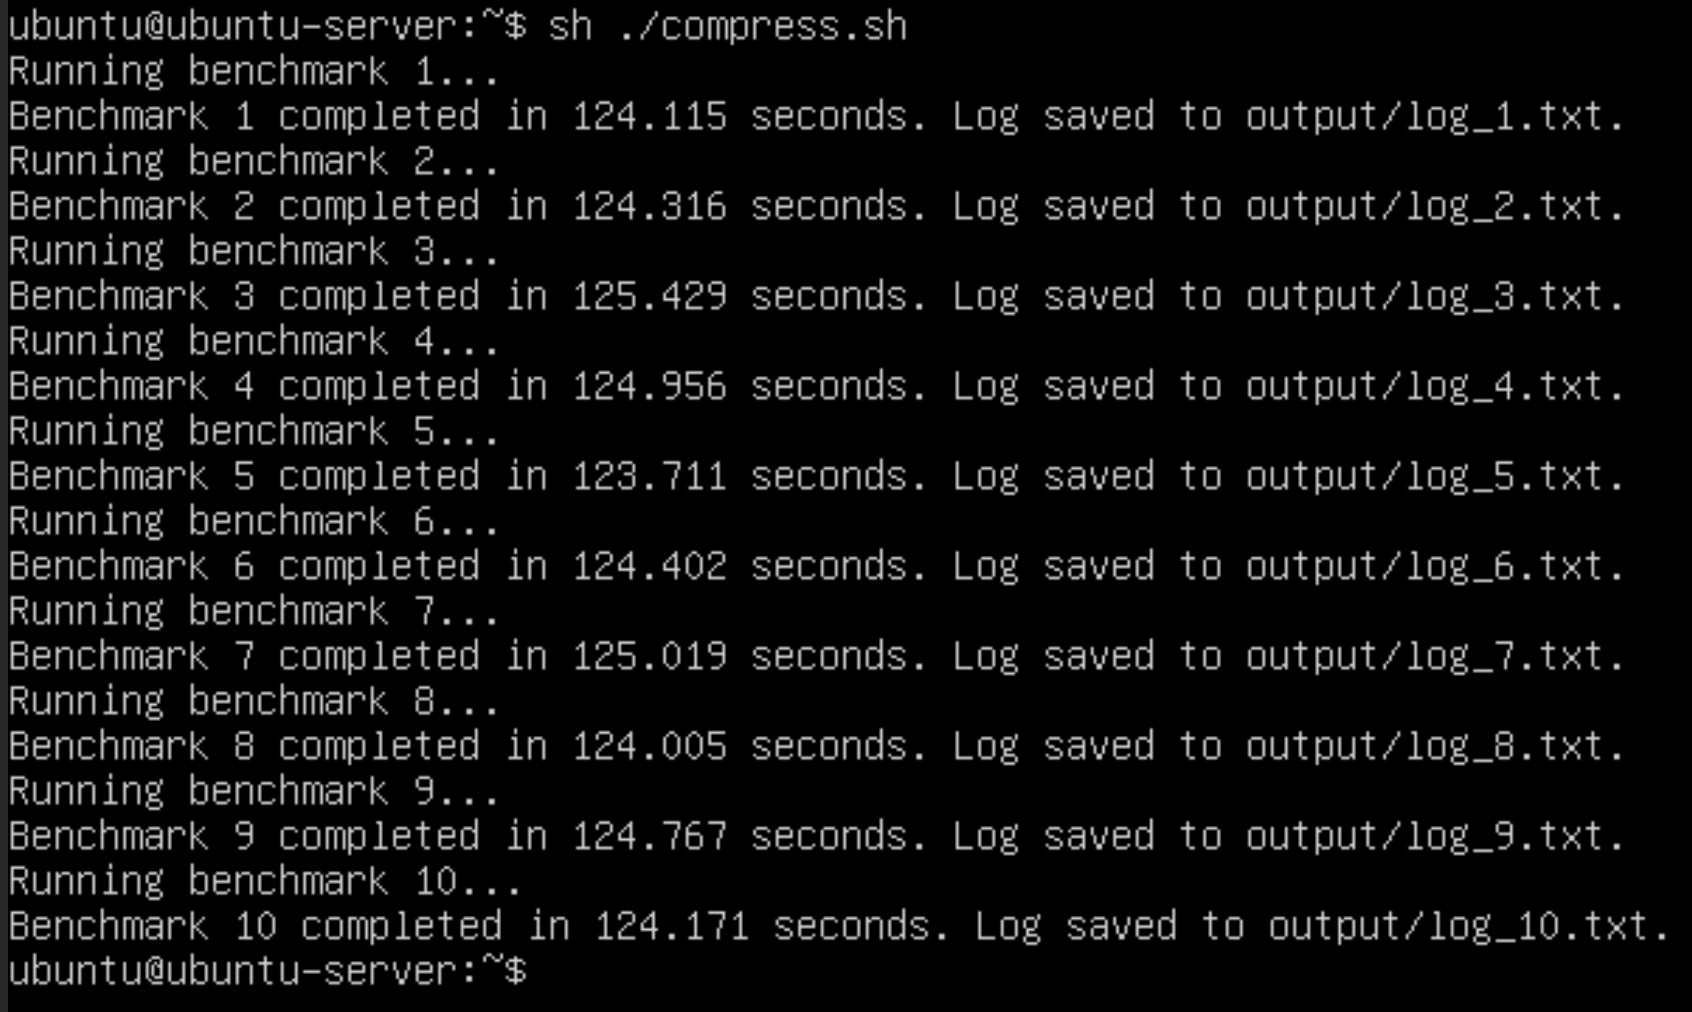
\includegraphics[width=1\textwidth]
    {assets/pics/video-compression-test/ssse3,sse4a.jpeg}
    \caption{Test Kompresi Video dengan Konfigurasi SSSE3 + SSE4a}
    \label{fig:video_compression_test_ssse3,sse4a}
\end{figure}

%-----------------------------------------------------------------------------%
\subsection{Konfigurasi dengan SSE4.1 + SSE4.2}
%-----------------------------------------------------------------------------%
\begin{figure}
    \centering
    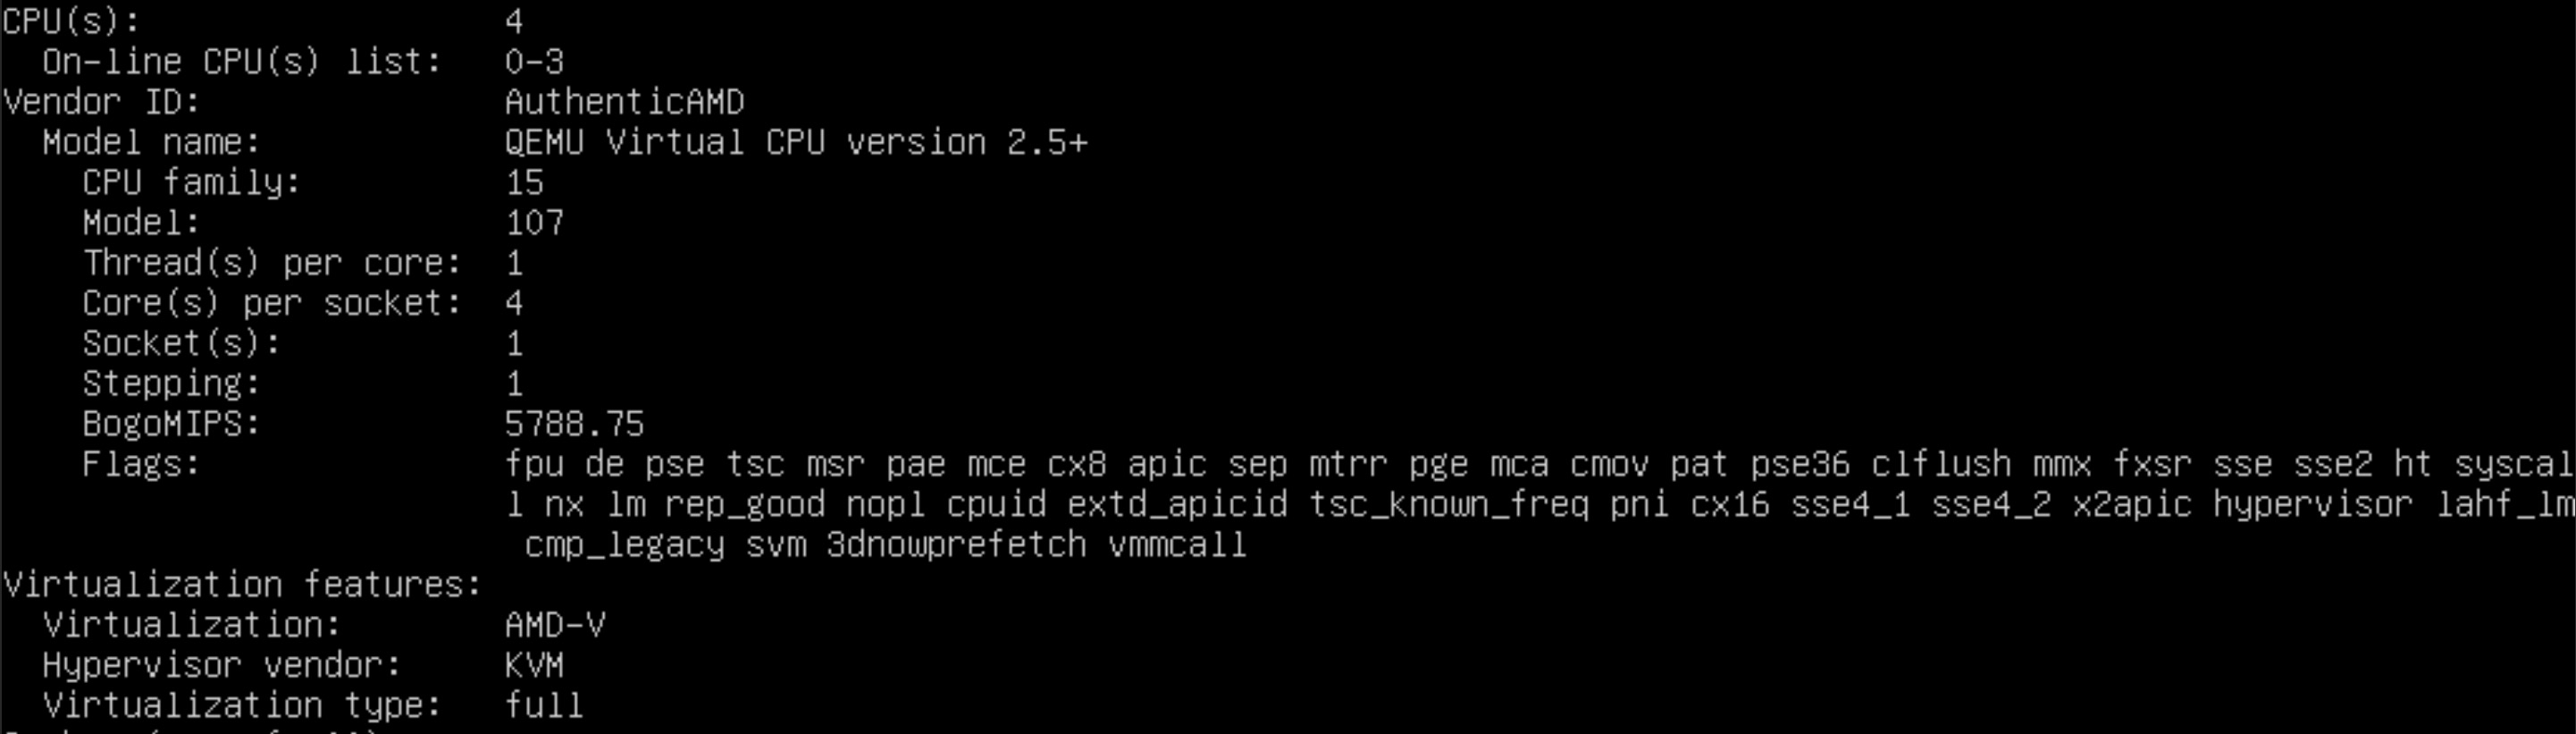
\includegraphics[width=1\textwidth]
    {assets/pics/video-compression-test/lscpu_sse4.1,sse4.2.jpeg}
    \caption{\texttt{lscpu} Konfigurasi SSE4.1 + SSE4.2}
    \label{fig:lscpu_video_compression_test_sse4.1,sse4.2}
\end{figure}

\begin{figure}
    \centering
    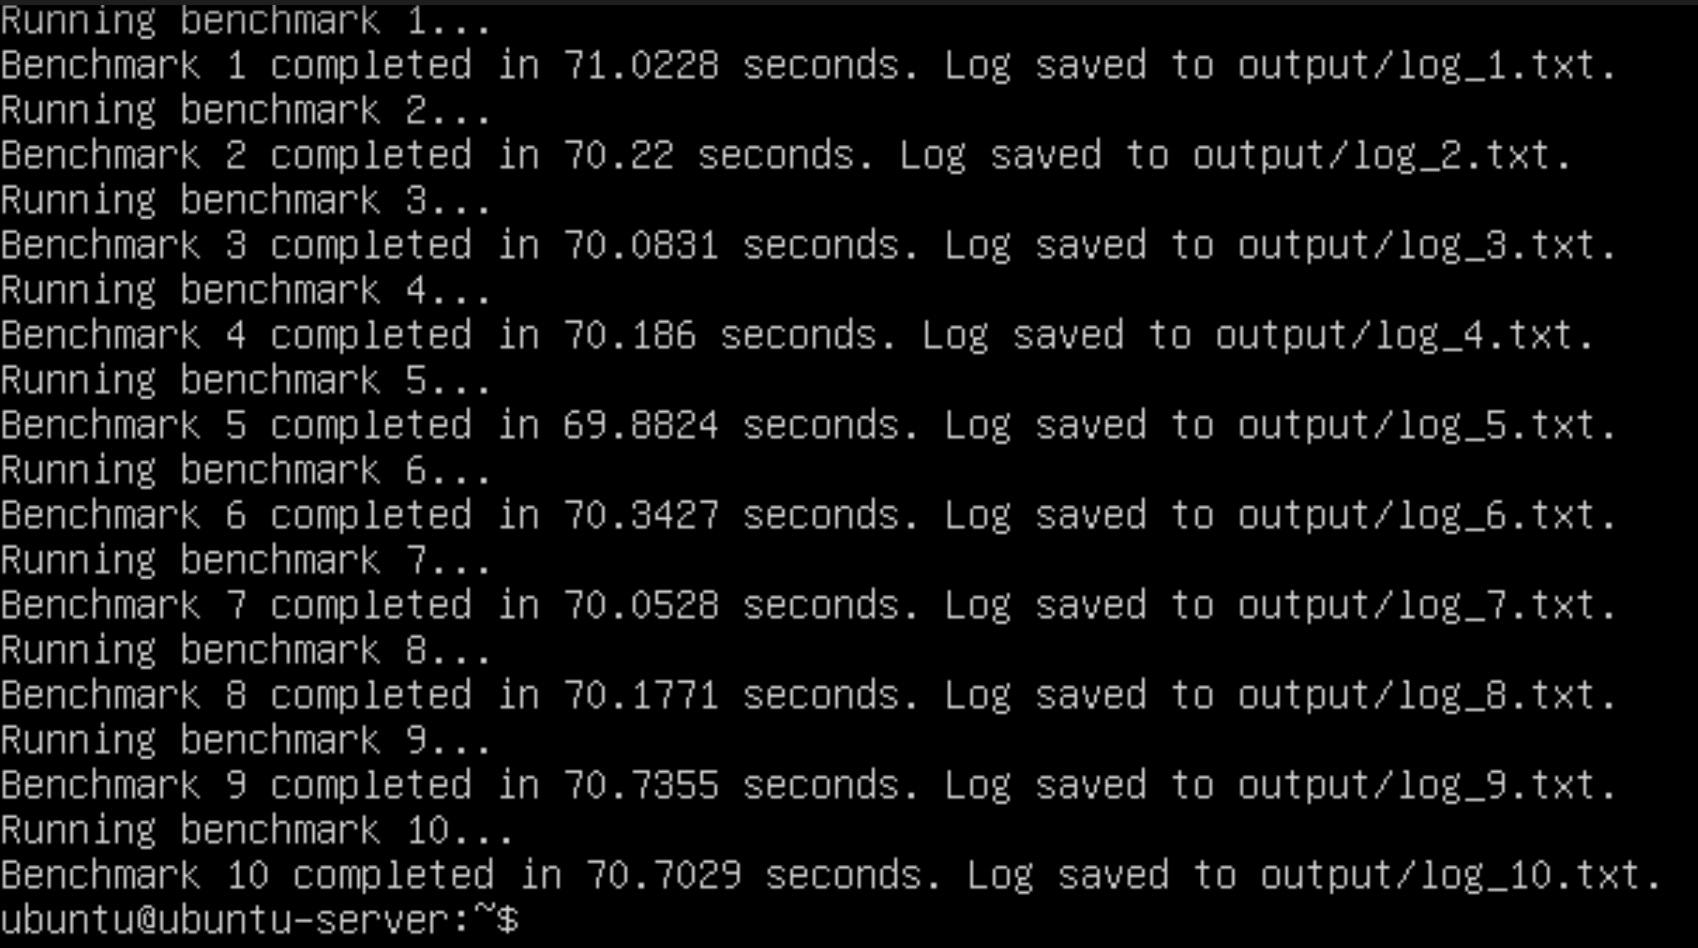
\includegraphics[width=1\textwidth]
    {assets/pics/video-compression-test/sse4.1,sse4.2.jpeg}
    \caption{Test Kompresi Video dengan Konfigurasi SSE4.1 + SSE4.2}
    \label{fig:video_compression_test_sse4.1,sse4.2}
\end{figure}

%-----------------------------------------------------------------------------%
\subsection{Konfigurasi dengan SSE4.1 + SSE4a}
%-----------------------------------------------------------------------------%
\begin{figure}
    \centering
    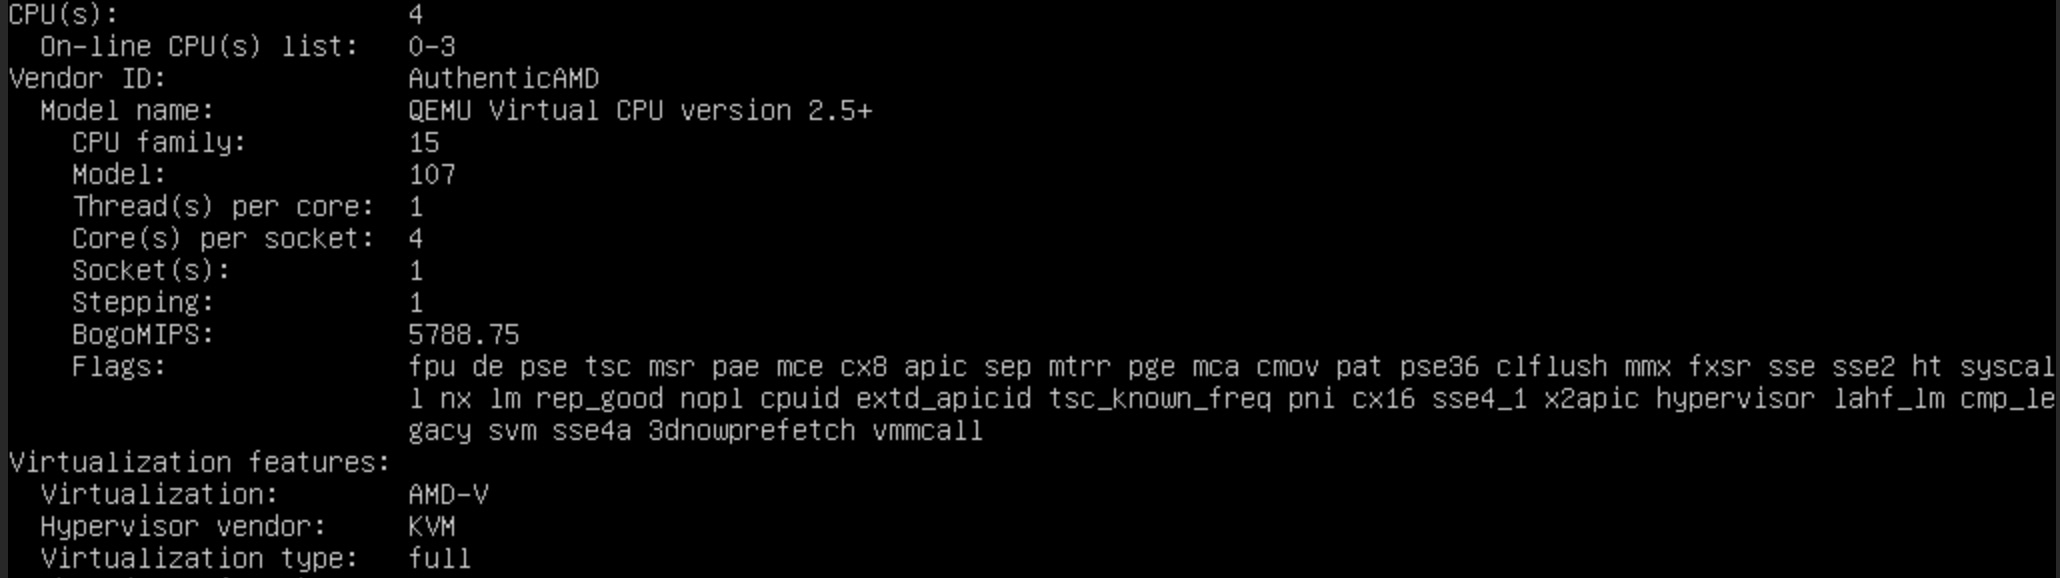
\includegraphics[width=1\textwidth]
    {assets/pics/video-compression-test/lscpu_sse4.1,sse4a.jpeg}
    \caption{\texttt{lscpu} Konfigurasi SSE4.1 + SSE4a}
    \label{fig:lscpu_video_compression_test_sse4.1,sse4a}
\end{figure}

\begin{figure}
    \centering
    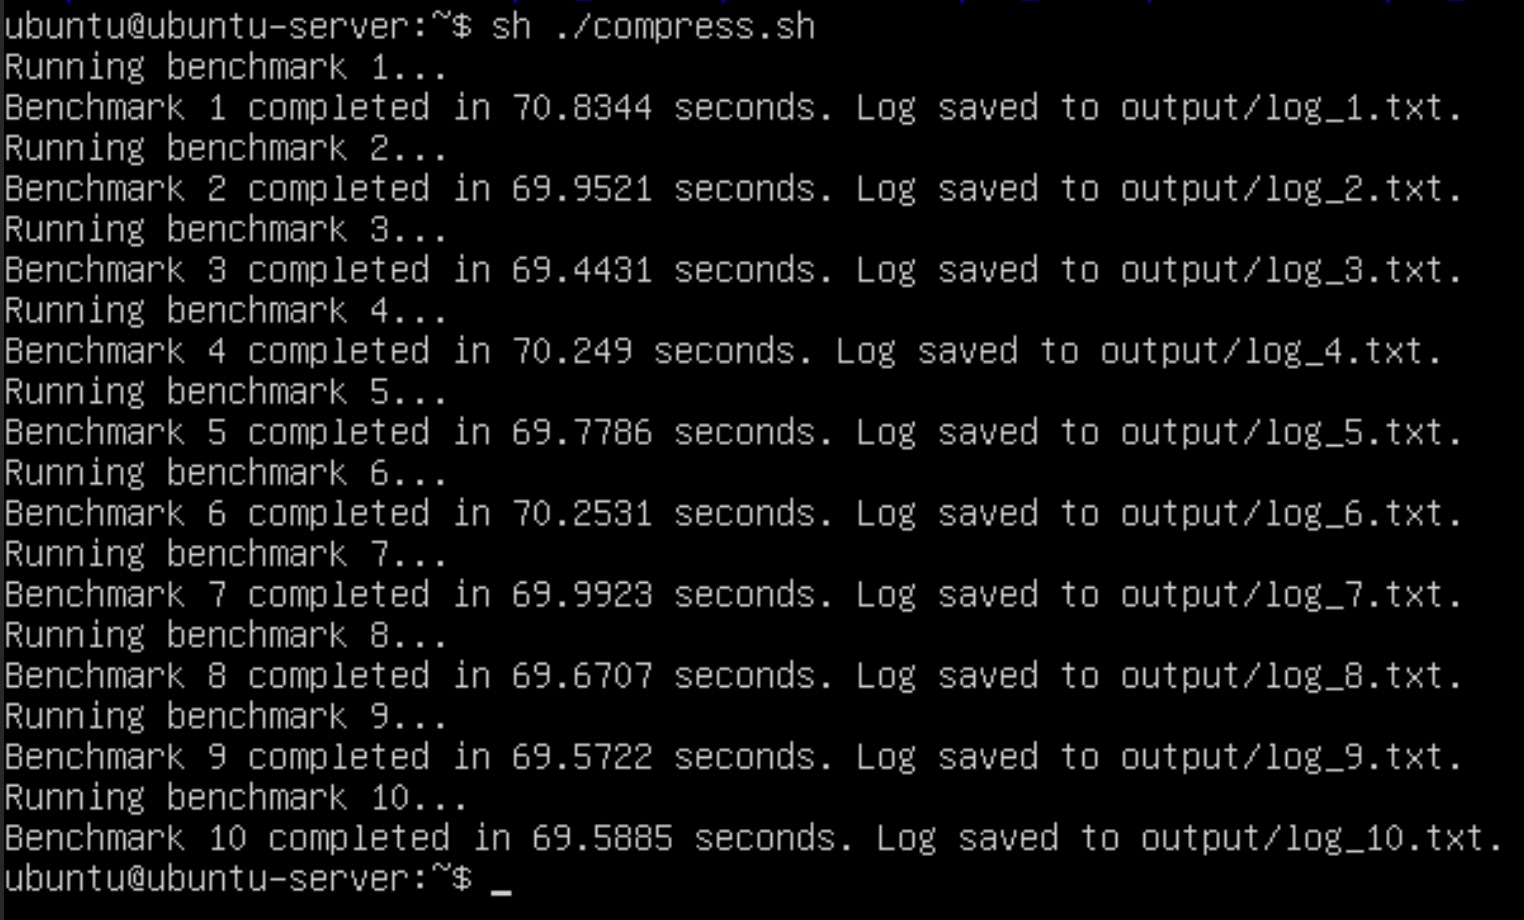
\includegraphics[width=1\textwidth]
    {assets/pics/video-compression-test/sse4.1,sse4a.jpeg}
    \caption{Test Kompresi Video dengan Konfigurasi SSE4.1 + SSE4a}
    \label{fig:video_compression_test_sse4.1,sse4a}
\end{figure}

%-----------------------------------------------------------------------------%
\subsection{Konfigurasi dengan SSE4.2 + SSE4a}
%-----------------------------------------------------------------------------%
\begin{figure}
    \centering
    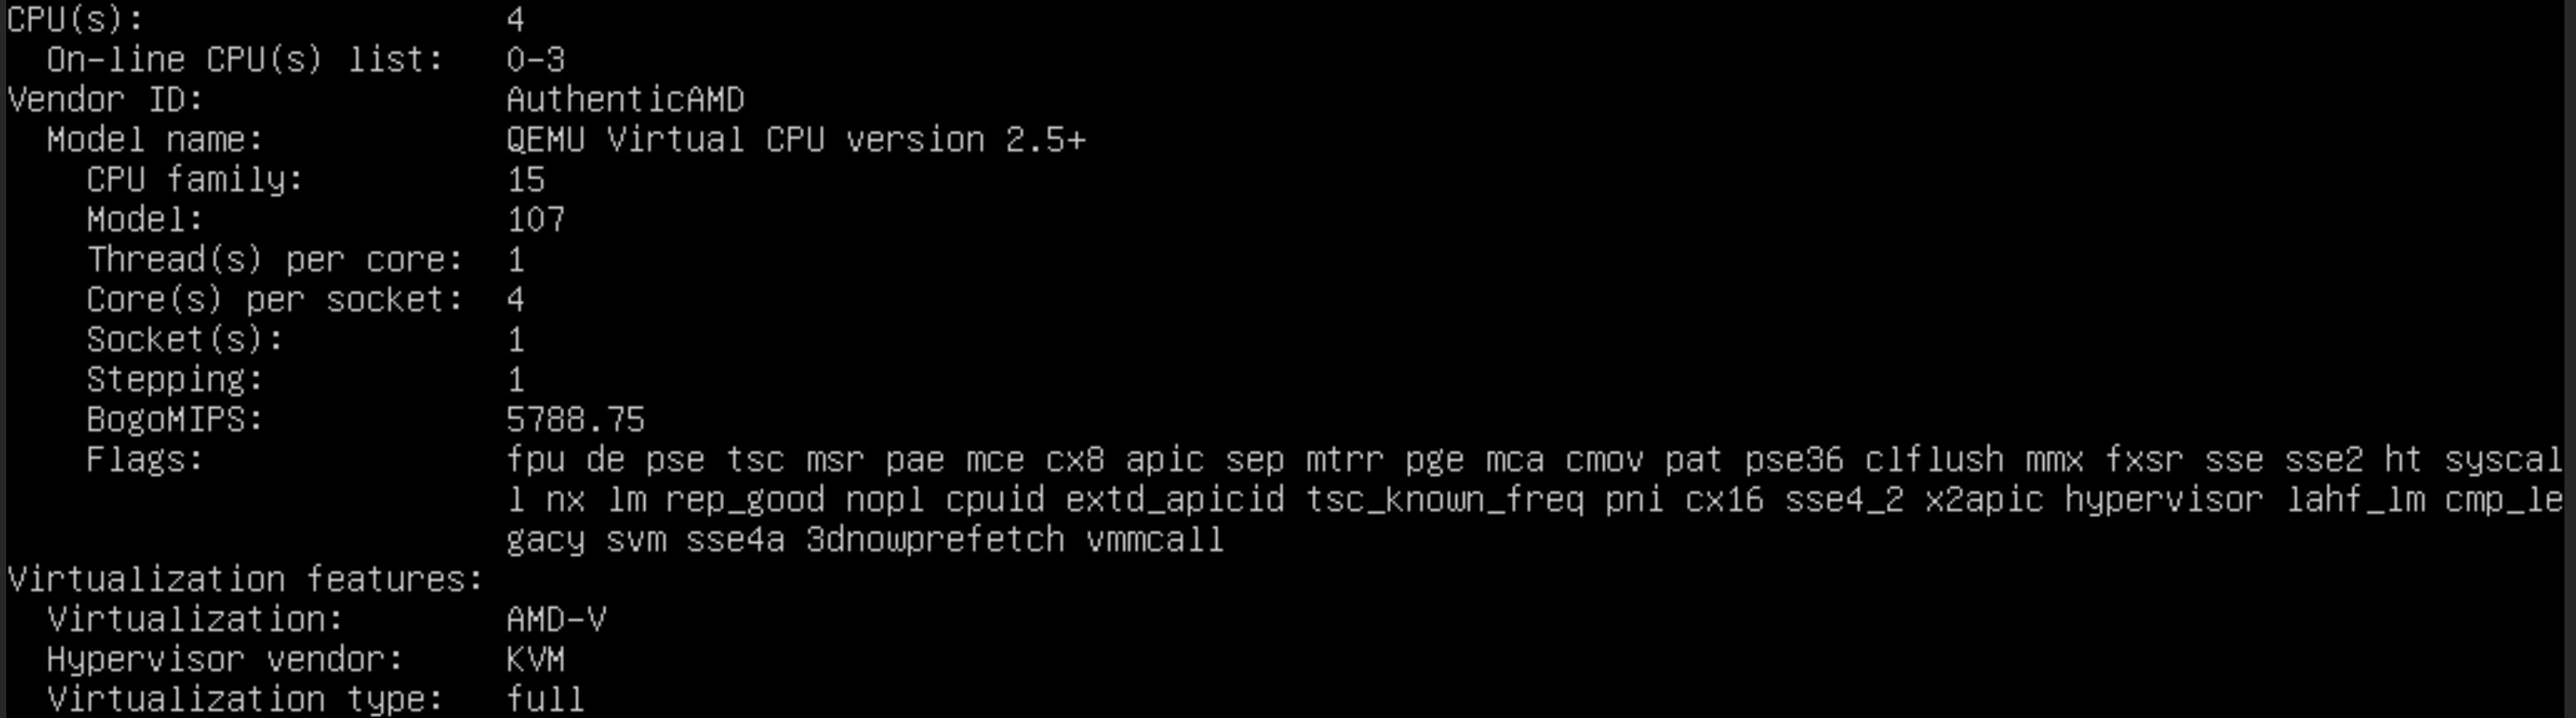
\includegraphics[width=1\textwidth]
    {assets/pics/video-compression-test/lscpu_sse4.2,sse4a.jpeg}
    \caption{\texttt{lscpu} Konfigurasi SSE4.2 + SSE4a}
    \label{fig:lscpu_video_compression_test_sse4.2,sse4a}
\end{figure}

\begin{figure}
    \centering
    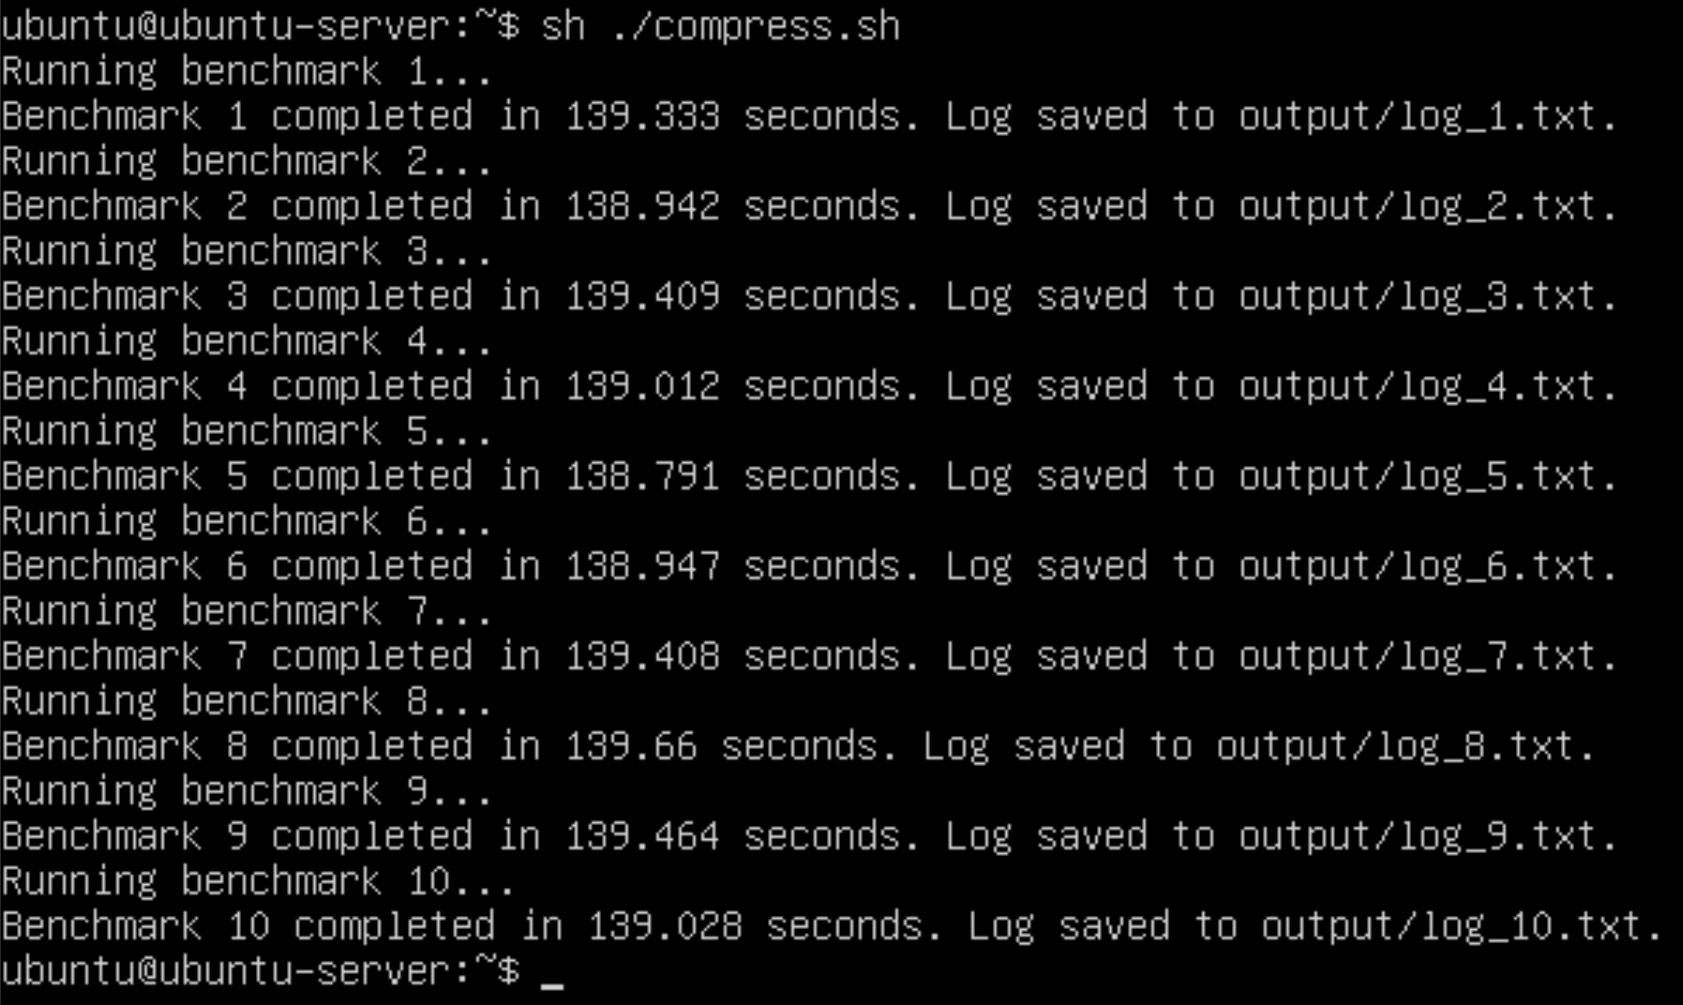
\includegraphics[width=1\textwidth]
    {assets/pics/video-compression-test/sse4.2,sse4a.jpeg}
    \caption{Test Kompresi Video dengan Konfigurasi SSE4.2 + SSE4a}
    \label{fig:video_compression_test_sse4.2,sse4a}
\end{figure}

%-----------------------------------------------------------------------------%
\subsection{Konfigurasi dengan SSSE3 + SSE4.1 + SSE4.2}
%-----------------------------------------------------------------------------%
% \begin{figure}
%     \centering
%     \includegraphics[width=1\textwidth]
%     {assets/pics/video-compression-test/lscpu_ssse3,sse4.1,sse4.2.jpeg}
%     \caption{\texttt{lscpu} Konfigurasi SSSE3 + SSE4.1 + SSE4.2}
%     \label{fig:lscpu_video_compression_test_ssse3,sse4.1,sse4.2}
% \end{figure}

\begin{figure}
    \centering
    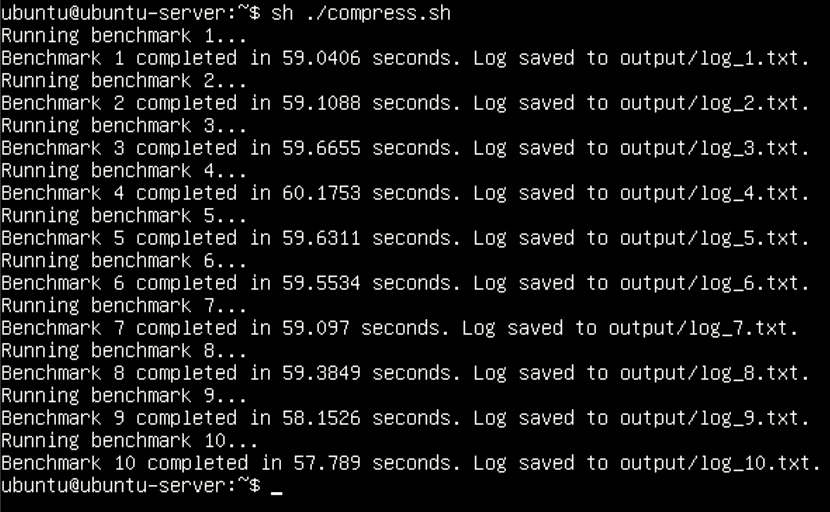
\includegraphics[width=1\textwidth]
    {assets/pics/video-compression-test/ssse3,sse4.1,sse4.2.jpeg}
    \caption{Test Kompresi Video dengan Konfigurasi SSSE3 + SSE4.1 + SSE4.2}
    \label{fig:video_compression_test_ssse3,sse4.1,sse4.2}
\end{figure}

%-----------------------------------------------------------------------------%
\subsection{Konfigurasi dengan SSSE3 + SSE4.1 + SSE4a}
%-----------------------------------------------------------------------------%
\begin{figure}
    \centering
    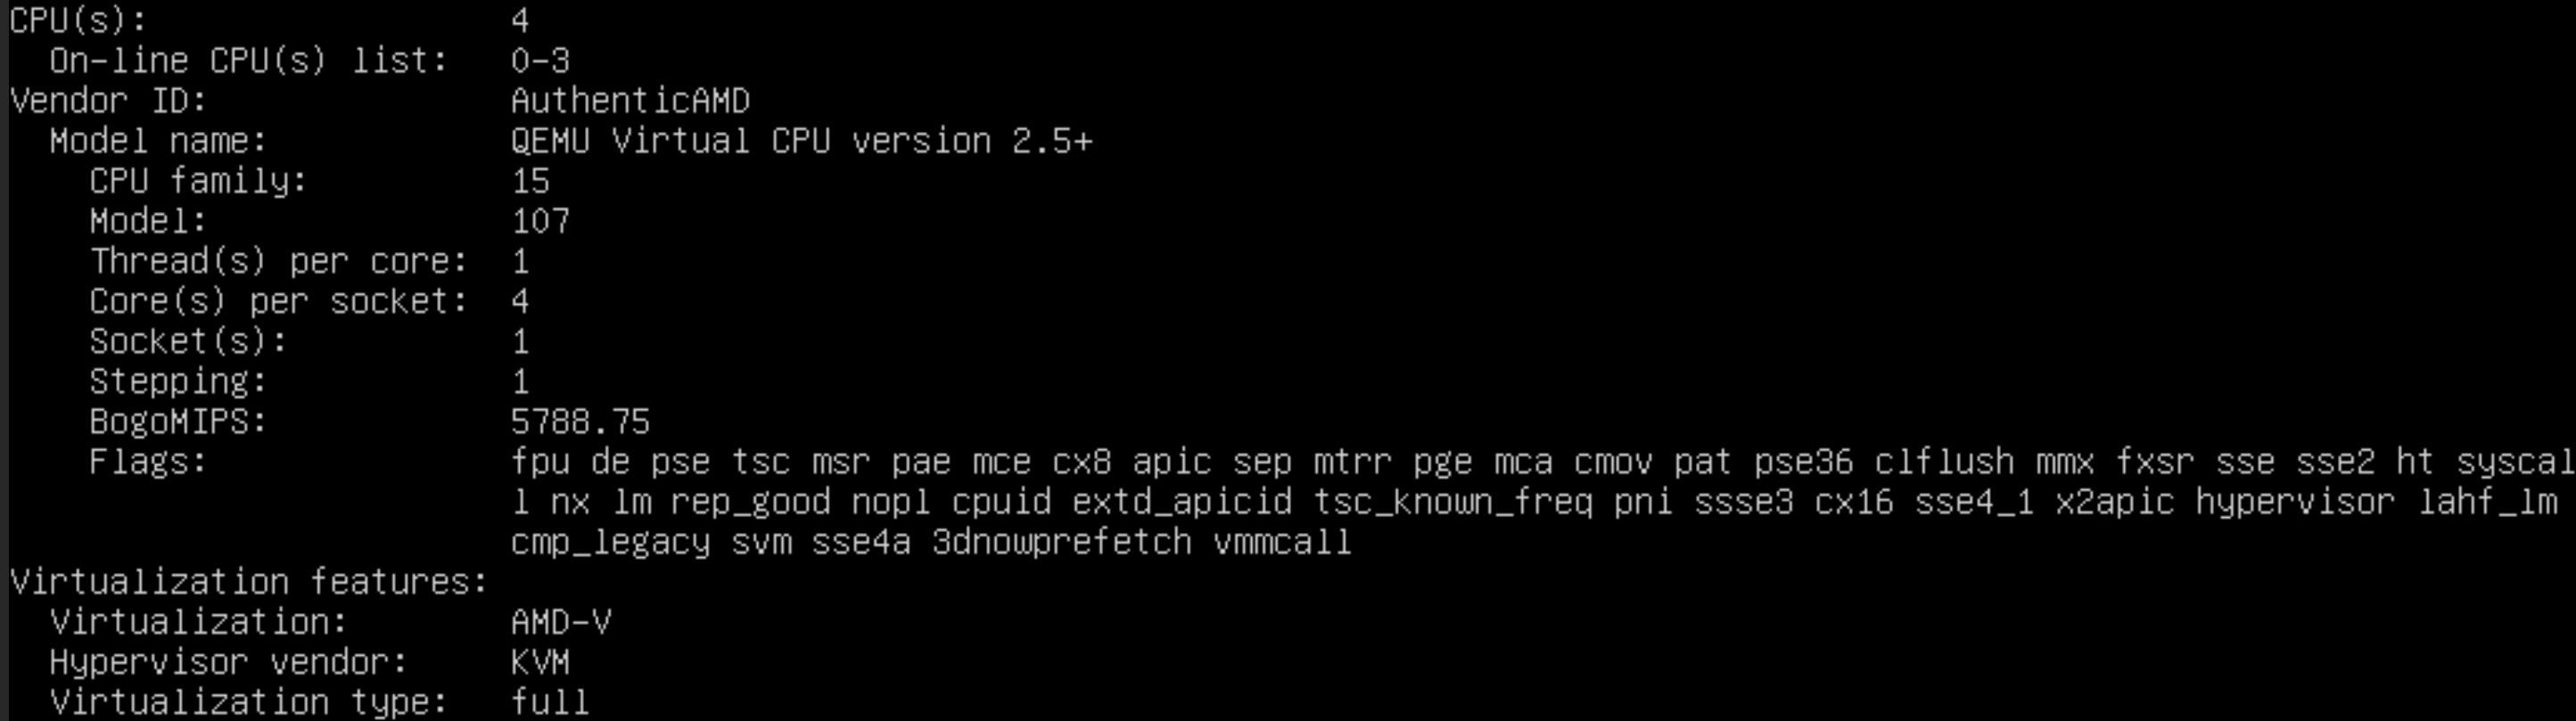
\includegraphics[width=1\textwidth]
    {assets/pics/video-compression-test/lscpu_ssse3,sse4.1,sse4a.jpeg}
    \caption{\texttt{lscpu} Konfigurasi SSSE3 + SSE4.1 + SSE4a}
    \label{fig:lscpu_video_compression_test_ssse3,sse4.1,sse4a}
\end{figure}

\begin{figure}
    \centering
    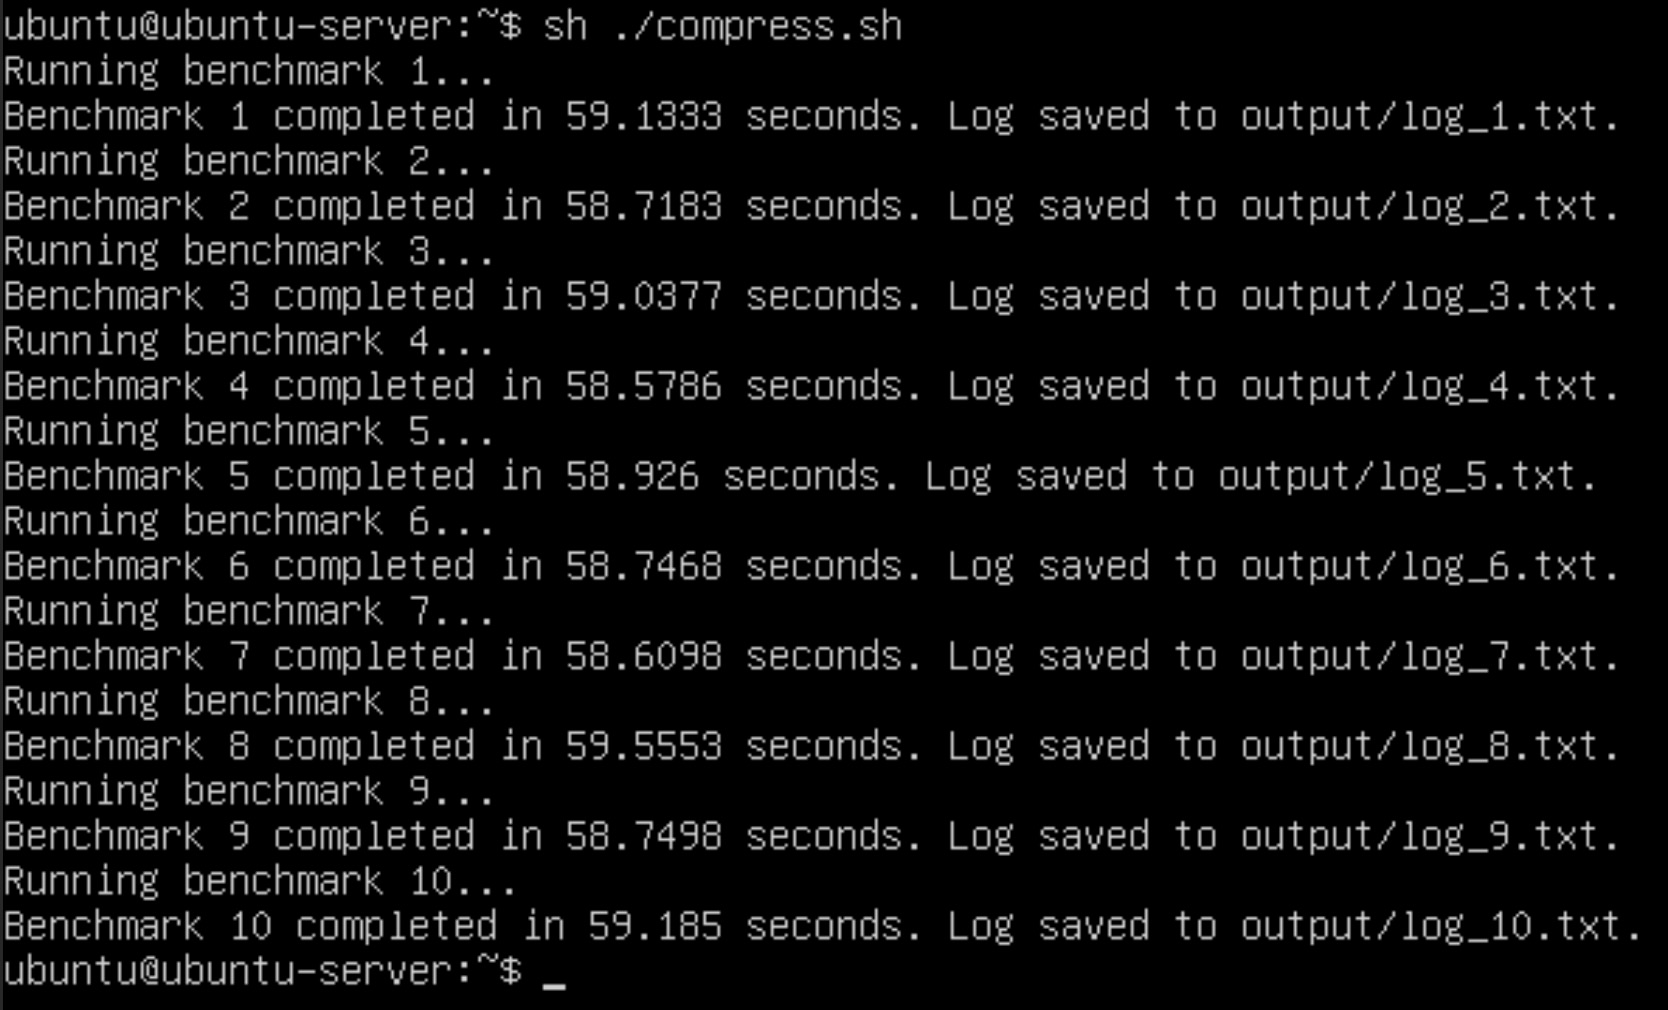
\includegraphics[width=1\textwidth]
    {assets/pics/video-compression-test/ssse3,sse4.1,sse4a.jpeg}
    \caption{Test Kompresi Video dengan Konfigurasi SSSE3 + SSE4.1 + SSE4a}
    \label{fig:video_compression_test_ssse3,sse4.1,sse4a}
\end{figure}

%-----------------------------------------------------------------------------%
\subsection{Konfigurasi dengan SSSE3 + SSE4.2 + SSE4a}
%-----------------------------------------------------------------------------%
\begin{figure}
    \centering
    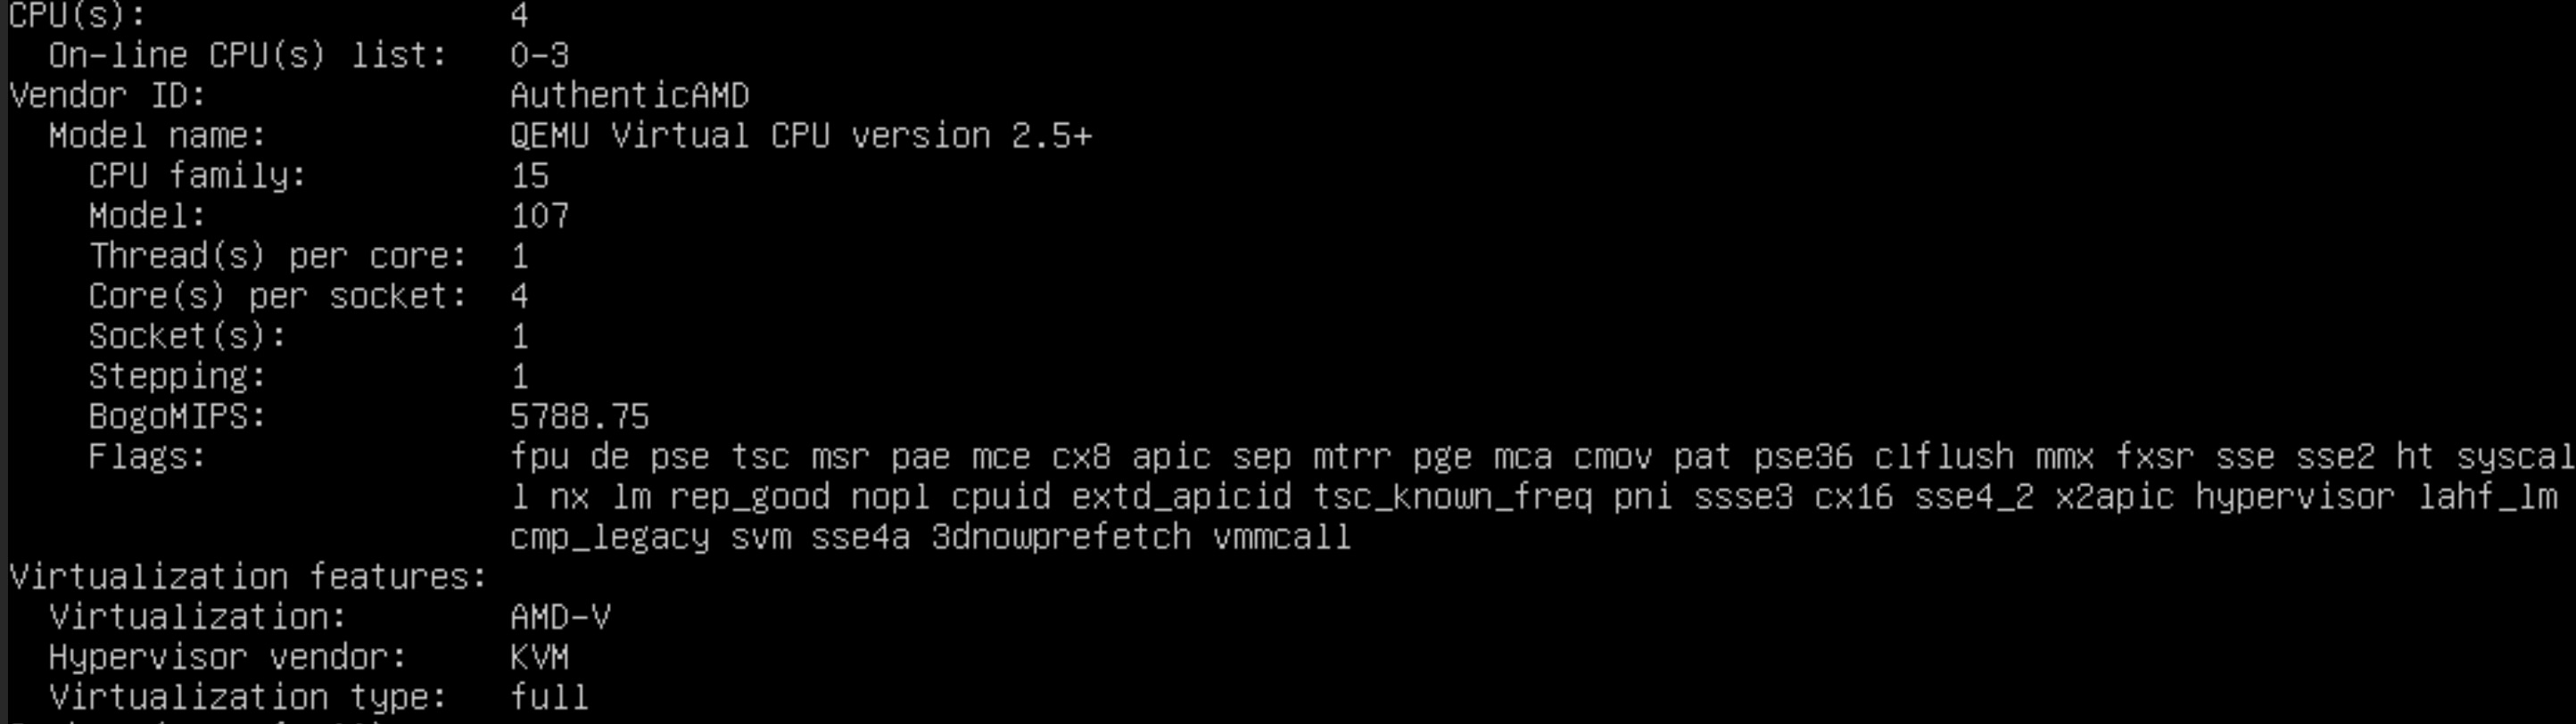
\includegraphics[width=1\textwidth]
    {assets/pics/video-compression-test/lscpu_ssse3,sse4.2,sse4a.jpeg}
    \caption{\texttt{lscpu} Konfigurasi SSSE3 + SSE4.2 + SSE4a}
    \label{fig:lscpu_video_compression_test_ssse3,sse4.2,sse4a.jpeg}
\end{figure}

\begin{figure}
    \centering
    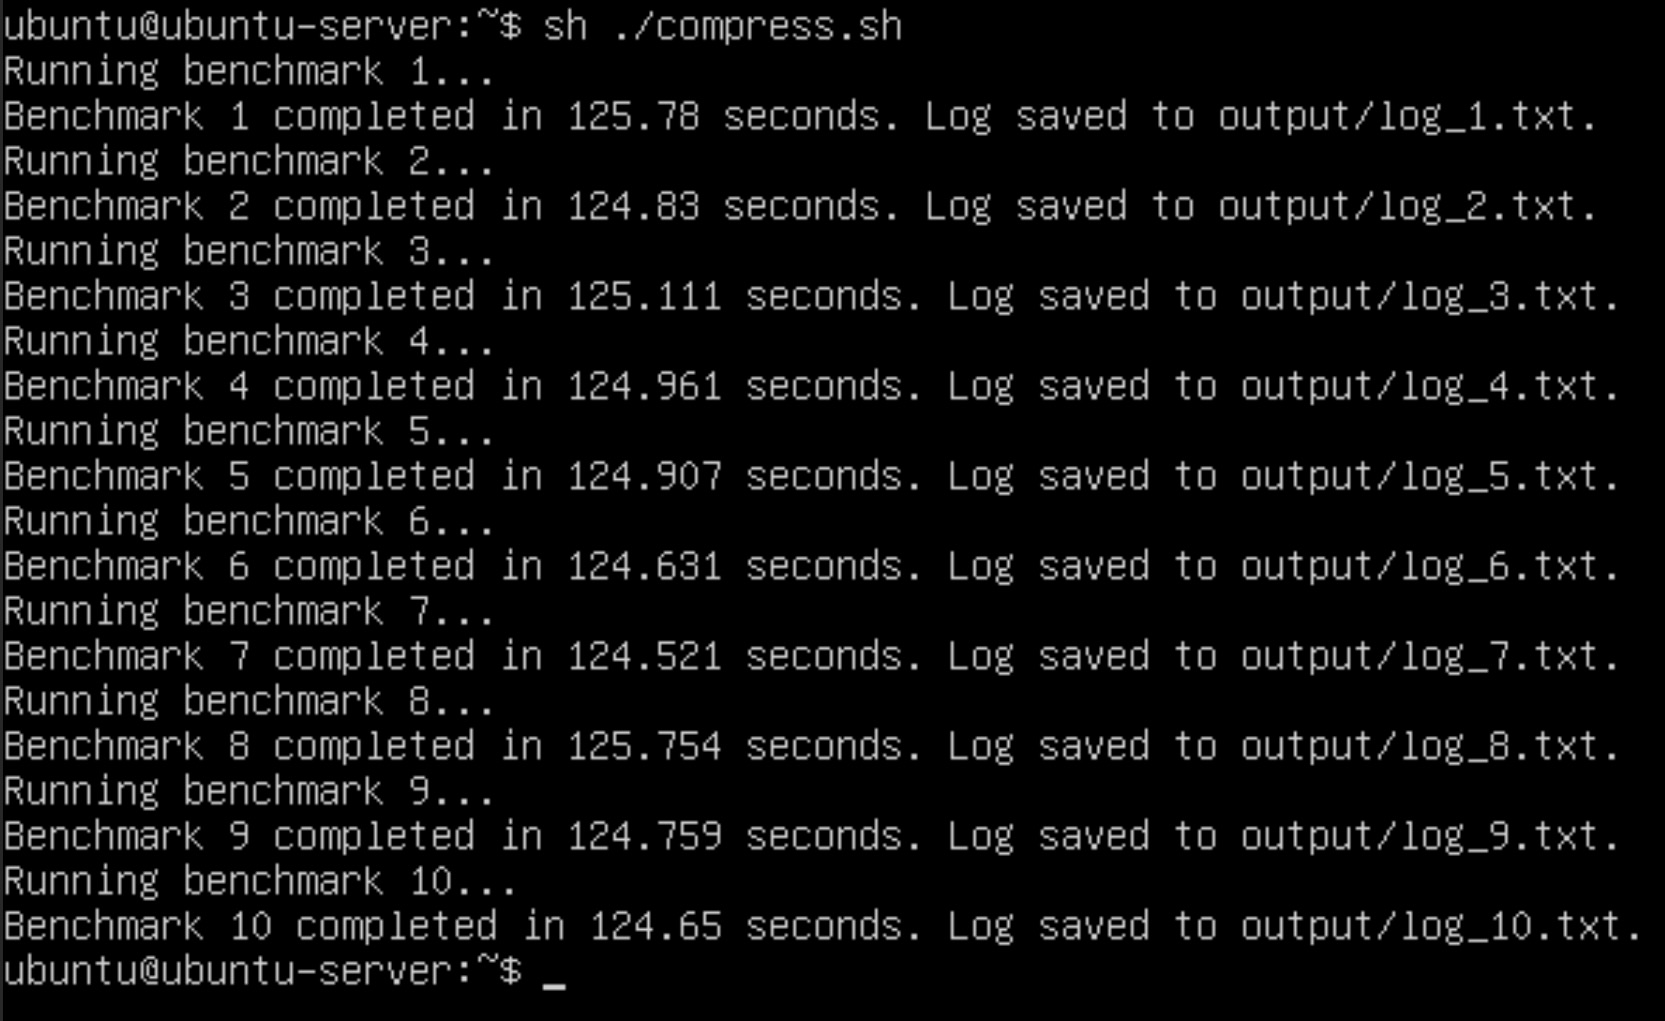
\includegraphics[width=1\textwidth]
    {assets/pics/video-compression-test/ssse3,sse4.2,sse4a.jpeg}
    \caption{Test Kompresi Video dengan Konfigurasi SSSE3 + SSE4.2 + SSE4a}
    \label{fig:video_compression_test_ssse3,sse4.2,sse4a.jpeg}
\end{figure}

%-----------------------------------------------------------------------------%
\subsection{Konfigurasi dengan SSE4.1 + SSE4.2 + SSE4a}
%-----------------------------------------------------------------------------%
\begin{figure}
    \centering
    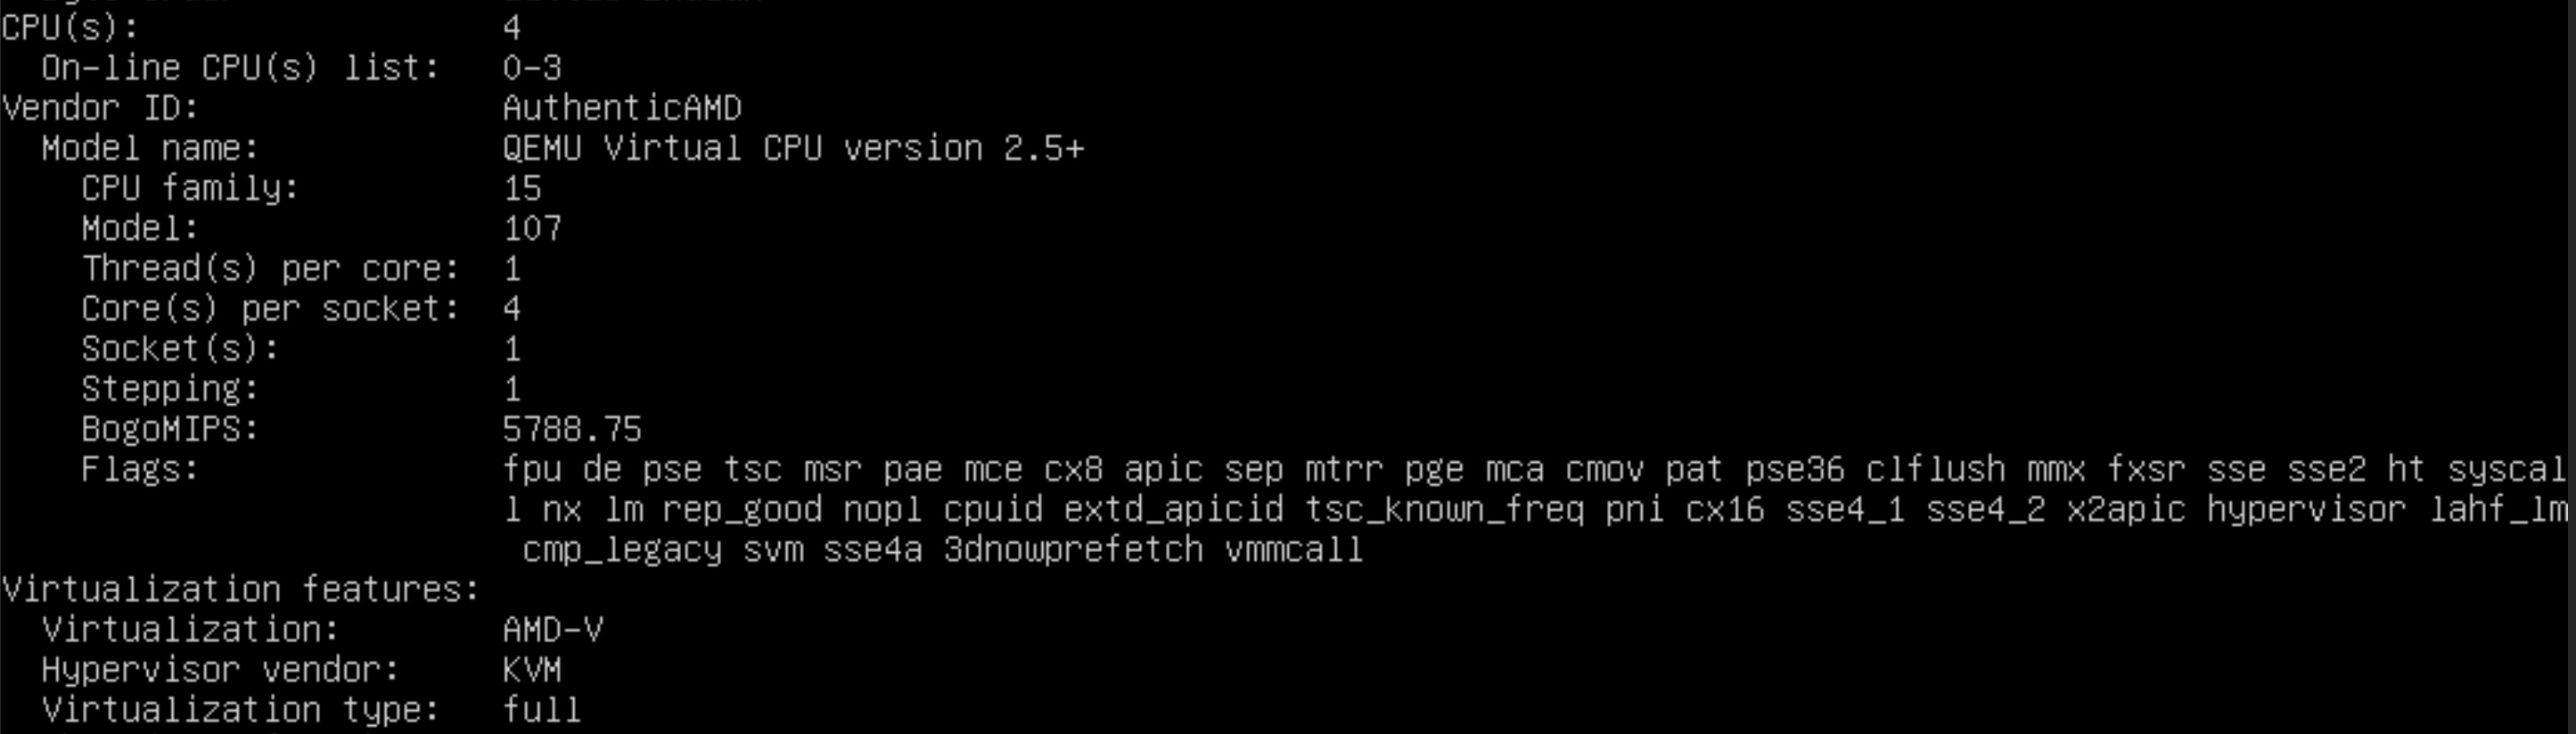
\includegraphics[width=1\textwidth]
    {assets/pics/video-compression-test/lscpu_sse4.1,sse4.2,sse4a.jpeg}
    \caption{\texttt{lscpu} Konfigurasi SSE4.1 + SSE4.2 + SSE4a}
    \label{fig:lscpu_video_compression_test_sse4.1,sse4.2,sse4a.jpeg}
\end{figure}

\begin{figure}
    \centering
    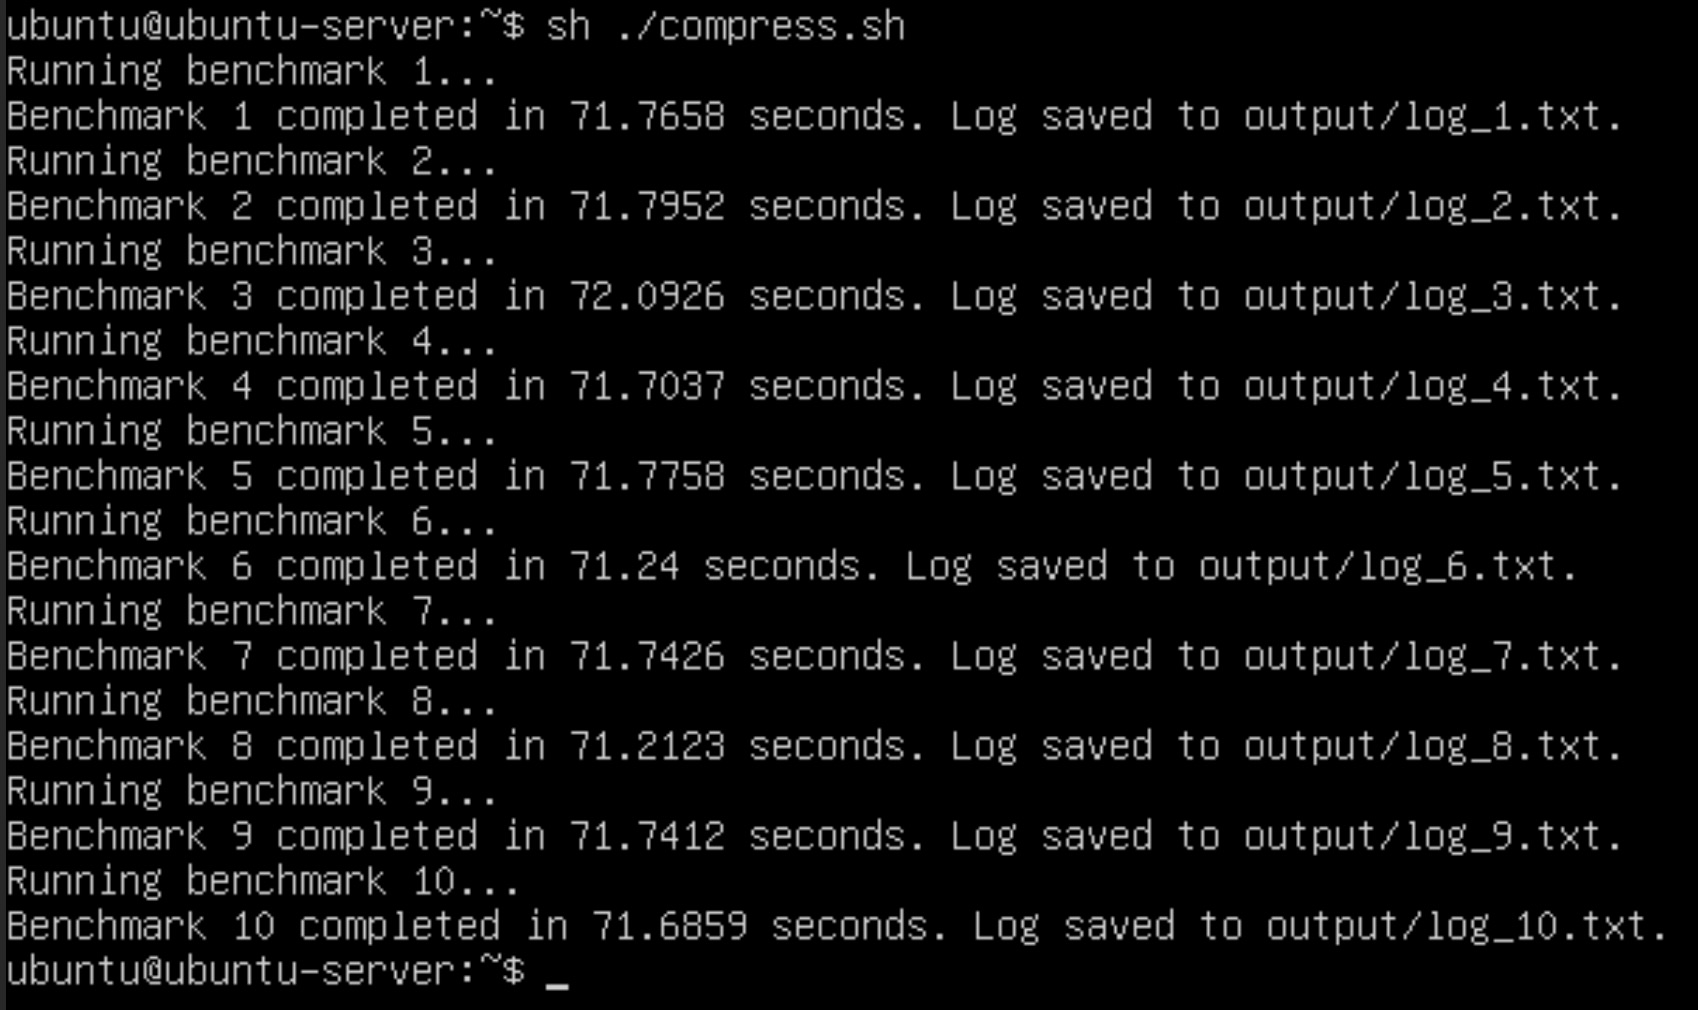
\includegraphics[width=1\textwidth]
    {assets/pics/video-compression-test/sse4.1,sse4.2,sse4a.jpeg}
    \caption{Test Kompresi Video dengan Konfigurasi SSE4.1 + SSE4.2 + SSE4a}
    \label{fig:video_compression_test_sse4.1,sse4.2,sse4a.jpeg}
\end{figure}

%-----------------------------------------------------------------------------%
\subsection{Konfigurasi dengan SSSE3 + SSE4.1 + SSE4.2 + SSE4a}
%-----------------------------------------------------------------------------%
% \begin{figure}
%     \centering
%     \includegraphics[width=1\textwidth]
%     {assets/pics/video-compression-test/lscpu_ssse3,sse4.1,sse4.2,sse4a.jpeg}
%     \caption{\texttt{lscpu} Konfigurasi SSSE3 + SSE4.1 + SSE4.2 + SSE4a}
%     \label{fig:lscpu_video_compression_test_ssse3,sse4.1,sse4.2,sse4a.jpeg}
% \end{figure}

\begin{figure}
    \centering
    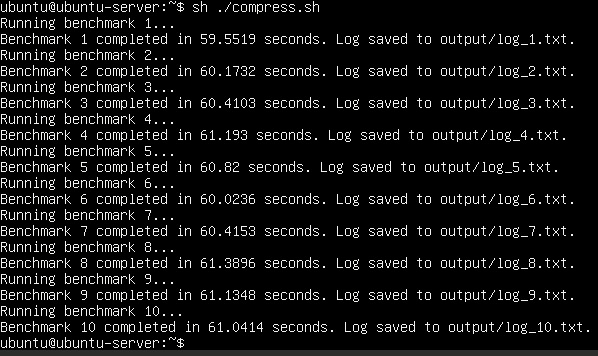
\includegraphics[width=1\textwidth]
    {assets/pics/video-compression-test/ssse3,sse4.1,sse4.2,sse4a.jpeg}
    \caption{Test Kompresi Video dengan Konfigurasi SSSE3 + SSE4.1 + SSE4.2 + SSE4a}
    \label{fig:video_compression_test_ssse3,sse4.1,sse4.2,sse4a.jpeg}
\end{figure}

%-----------------------------------------------------------------------------%
\subsection{Analisis Pengujian Tuning Hypervisor KVM dengan Kompresi Video}
%-----------------------------------------------------------------------------%

%-----------------------------------------------------------------------------%
\section{Hasil Pengujian Tuning Hypervisor KVM dengan Validasi Integraitas File}
%-----------------------------------------------------------------------------%

%-----------------------------------------------------------------------------%
\subsection{Konfigurasi Default}
%-----------------------------------------------------------------------------%

%-----------------------------------------------------------------------------%
\subsection{Konfigurasi dengan SSE4.2}
%-----------------------------------------------------------------------------%

%-----------------------------------------------------------------------------%
\subsection{Analisis Pengujian Tuning Hypervisor KVM dengan Validasi Integraitas File}
%-----------------------------------------------------------------------------%

%-----------------------------------------------------------------------------%
\section{Hasil Pengujian Tuning Hypervisor KVM dengan Enkripsi AES}
%-----------------------------------------------------------------------------%

%-----------------------------------------------------------------------------%
\subsection{Konfigurasi Default}
%-----------------------------------------------------------------------------%

%-----------------------------------------------------------------------------%
\subsection{Konfigurasi dengan AES}
%-----------------------------------------------------------------------------%

%-----------------------------------------------------------------------------%
\subsection{Analisis Pengujian Tuning Hypervisor KVM dengan Enkripsi AES}
%-----------------------------------------------------------------------------%


\iffalse
%-----------------------------------------------------------------------------%
%\chapter{\babEmpat}
%-----------------------------------------------------------------------------%
\todo{tambahkan kata-kata pengantar bab 1 disini}

%-----------------------------------------------------------------------------%
\section{thesis.tex}
%-----------------------------------------------------------------------------%
Berkas ini berisi seluruh berkas Latex yang dibaca, jadi bisa dikatakan sebagai 
berkas utama. Dari berkas ini kita dapat mengatur bab apa saja yang ingin 
kita tampilkan dalam dokumen.


%-----------------------------------------------------------------------------%
\section{laporan\_setting.tex}
%-----------------------------------------------------------------------------%
Berkas ini berguna untuk mempermudah pembuatan beberapa template standar. 
Anda diminta untuk menuliskan judul laporan, nama, npm, dan hal-hal lain yang 
dibutuhkan untuk pembuatan template. 


%-----------------------------------------------------------------------------%
\section{istilah.tex}
%-----------------------------------------------------------------------------%
Berkas istilah digunakan untuk mencatat istilah-istilah yang digunakan. 
Fungsinya hanya untuk memudahkan penulisan.
Pada beberapa kasus, ada kata-kata yang harus selalu muncul dengan tercetak 
miring atau tercetak tebal. 
Dengan menjadikan kata-kata tersebut sebagai sebuah perintah \latex~tentu akan 
mempercepat dan mempermudah pengerjaan laporan. 


%-----------------------------------------------------------------------------%
\section{hype.indonesia.tex}
%-----------------------------------------------------------------------------%
Berkas ini berisi cara pemenggalan beberapa kata dalam bahasa Indonesia. 
\latex~memiliki algoritma untuk memenggal kata-kata sendiri, namun untuk 
beberapa kasus algoritma ini memenggal dengan cara yang salah. 
Untuk memperbaiki pemenggalan yang salah inilah cara pemenggalan yang benar 
ditulis dalam berkas hype.indonesia.tex.


%-----------------------------------------------------------------------------%
\section{pustaka.tex}
%-----------------------------------------------------------------------------%
Berkas pustaka.tex berisi seluruh daftar referensi yang digunakan dalam 
laporan. 
Anda bisa membuat model daftar referensi lain dengan menggunakan bibtex.
Untuk mempelajari bibtex lebih lanjut, silahkan buka 
\url{http://www.bibtex.org/Format}. 
Untuk merujuk pada salah satu referensi yang ada, gunakan perintah \bslash 
cite, e.g. \bslash cite\{lankton2008introduction\} yang akan akan memunculkan 
\cite{lankton2008introduction}


%-----------------------------------------------------------------------------%
\section{bab[1 - 6].tex}
%-----------------------------------------------------------------------------%
Berkas ini berisi isi laporan yang Anda tulis. 
Setiap nama berkas e.g. bab1.tex merepresentasikan bab dimana tulisan tersebut 
akan muncul. 
Sebagai contoh, kode dimana tulisan ini dibaut berada dalam berkas dengan nama 
bab4.tex. 
Ada enam buah berkas yang telah disiapkan untuk mengakomodir enam bab dari 
laporan Anda, diluar bab kesimpulan dan saran. 
Jika Anda tidak membutuhkan sebanyak itu, silahkan hapus kode dalam berkas 
thesis.tex yang memasukan berkas \latex~yang tidak dibutuhkan;  contohnya 
perintah \bslash include\{bab6.tex\} merupakan kode untuk memasukan berkas 
bab6.tex kedalam laporan.

%-----------------------------------------------------------------------------%
\section{Penulisan \textit{code} atau \textit{pseudocode} program}
%-----------------------------------------------------------------------------%

\subsection{\textit{Inline}}

Dengan perintah \verb|\verb|: \verb|System.out.println("Hello, World");| \\
Dengan perintah \textit{custom} \verb|\code|: \code{System.out.println("Hello, World"); }
Dengan perintah \verb|\mintinline|: \mintinline{java}{System.out.println("Hello, World"); }

\subsection{\textit{Multiline}}

Dengan perintah \verb|verbatim|: 

\begin{verbatim}	
public class HelloWorld {
    public static void main(String[] args) {
        // Prints "Hello, World" to the terminal window.
        System.out.println("Hello, World");
    }
}
\end{verbatim}

Dengan perintah \verb|minted|: Kode \ref{code:hw:minted}
\begin{listing}[H]
    \begin{minted}{python}
def binary_accuracy(y_true, y_pred):
    return K.mean(K.equal(y_true, K.round(y_pred)), axis=-1)


def categorical_accuracy(y_true, y_pred):
    return K.cast(K.equal(K.argmax(y_true, axis=-1),
                          K.argmax(y_pred, axis=-1)),
                  K.floatx())


def sparse_categorical_accuracy(y_true, y_pred):
    # reshape in case it's in shape (num_samples, 1) instead of (num_samples,)
    if K.ndim(y_true) == K.ndim(y_pred):
        y_true = K.squeeze(y_true, -1)
    # convert dense predictions to labels
    y_pred_labels = K.argmax(y_pred, axis=-1)
    y_pred_labels = K.cast(y_pred_labels, K.floatx())
    return K.cast(K.equal(y_true, y_pred_labels), K.floatx())


def top_k_categorical_accuracy(y_true, y_pred, k=5):
    return K.mean(K.in_top_k(y_pred, K.argmax(y_true, axis=-1), k), axis=-1)


def sparse_top_k_categorical_accuracy(y_true, y_pred, k=5):
    # If the shape of y_true is (num_samples, 1), flatten to (num_samples,)
    return K.mean(K.in_top_k(y_pred, K.cast(K.flatten(y_true), 'int32'), k),
                  axis=-1)
    \end{minted}
    \caption{An excerpt from keras: \url{https://github.com/keras-team/keras/blob/master/keras/metrics.py}}
    \label{code:hw:minted}
\end{listing}

Konfigurasi tampilan bisa dilakukan di \verb|uithesis.sty| dengan referensi dokumentasi di \url{https://github.com/gpoore/minted/blob/master/source/minted.pdf}

\fi